% !TeX root = ../../Book3.tex
% 纲要标题：## 第7章　Rauch、Riccati 与距离函数比较
% 纲要位置：几何学计划纲要.md，第 2359 行。
% 正文状态：初稿；尚未正式审核。

% 纲要内容开始
% 
% > 本章目标与证明范围：比较定理按共同初值、有效区间、不等式方向与等号条件组织。由 Jacobi 场逐步转为 Hessian、Laplace 和体积密度，而非并列罗列四个定理。
% 
% 纲要内容结束

\chapter{Rauch、Riccati 与距离函数比较}
\label{g3:ch:07}
\BookChapterNumber{g3:ch:07}

\begin{chapterabstract}
	曲率界怎样控制从同一点发出的测地线的分离速度？本章先用指标形式的极小性比较 Jacobi 场，得到常曲率模型的 Rauch 比较及指数映射微分估计；再将二阶 Jacobi 方程改写成矩阵 Riccati 方程，通过取迹与平方和估计导出 Ricci 曲率下界所控制的量。径向算子随后被识别为距离函数的 Hessian，迹与行列式分别给出 Laplace 和体积密度比较。最后处理割迹处的光滑支撑和分布不等式，并从等号恢复局部常曲率度量。
\end{chapterabstract}

\begin{learninggoals}
	\begin{itemize}
		\item 在共同初值及有效半径内比较 Jacobi 场，判断曲率界与长度估计的方向。
		\item 推导径向 Riccati 方程、奇异初值与迹不等式，解释各个等号条件。
		\item 将径向 Jacobi 数据转成距离 Hessian、Laplace 与极坐标密度。
		\item 构造割点处的光滑上支撑，并用极坐标分部积分证明分布比较。
		\item 说明单个方向的等号控制什么，以及哪些等号足以恢复一个常曲率球。
	\end{itemize}
\end{learninggoals}

在 Euclid 平面上，两条初始夹角很小的射线，距离起点越远，彼此的横向间距越大，且一阶间距随半径线性增长。在圆球面上，从北极出发的经线却会逐渐靠拢，最终在南极相遇；双曲平面的相应间距增长得比线性更快。第六章已经用 Jacobi 方程精确计算了这三个模型。现在考虑曲率不恒定的流形：若只知道截面曲率夹在两个常数之间，还能否用这些模型夹住测地线的分离量？

\ProseParagraphBreak

比较 Jacobi 方程的系数还不够。向量的方向也会变化，区间终点可能已经越过共轭点，而距离函数还会在割点失去光滑性。我们先在同一参数长度、同类初始或端点条件下比较指标形式，再沿射线积分得到长度估计。把一族 Jacobi 场的导数乘以其值矩阵的逆，可以直接研究径向伸缩率；这一变化把二阶线性方程转成一阶矩阵 Riccati 方程。取迹以后，截面曲率的逐方向控制被 Ricci 曲率的总和控制所替代，所得结论也相应由 Hessian 比较变成 Laplace 比较。

\ProseParagraphBreak

直接所需基础是第二章的指数映射、最短线及割时，第三章的曲率与 Hessian，第六章的 Jacobi 初值问题、指标引理和共轭点判别。最后一节使用一元绝对连续函数的积分分部、Fubini 与坐标换元，并在使用处建立距离函数所需的弱导数解释。延伸阅读可查 Petersen 第三版的 Riccati 与共轭半径比较，以及 Ricci 比较的基本方程和支撑函数方法\cite[第6.4.1--6.4.2节，第7.1.1节，第7.1.3--7.1.4节]{Petersen2016}。本章始终保留第一章的非负 Laplace 约定 \(\Delta=-\operatorname{div}\operatorname{grad}\)，因此文献中以 \(\operatorname{div}\operatorname{grad}\) 表示的距离上界，在本书中写成 \(\Delta r\) 的下界。

% !TeX root = ../../Book3.tex
% 纲要标题：### 7.1 指标形式的比较方法
% 纲要位置：几何学计划纲要.md，第 2363 行。
% 正文状态：初稿；尚未正式审核。

% 纲要内容开始
% 
% * 模型 Jacobi 场
% * 相同端点条件与变分极小性
% * Rauch 比较的证明
% * 共轭半径和微分长度估计
% 
% 纲要内容结束

\section{指标形式的比较方法}
\label{g3:sec:0701}

第六章把相邻测地线的分离写成 Jacobi 方程。常曲率时，方程有正弦、线性和双曲正弦三类显式解；一般流形上的曲率随位置与方向变化，很少能直接求解。比较方法保留相同初值，用曲率界代替完整的曲率函数，进而把未知解的长度夹在模型解之间。本节证明 Rauch\footnote{Harry Ernest Rauch（1925--1979），美国数学家，研究黎曼几何与复分析，在曲率夹逼、黎曼曲面及 theta 函数理论方面作出贡献。} 比较定理与常曲率模型比较的版本。关键工具是上一章的指标极小性质：在没有共轭点的区间内，Jacobi 场使给定端点值的指标形式最小。

\subsection{模型 Jacobi 场}
\label{g3:subsec:0701:01}

本节设黎曼流形光滑、无边界，测地线均用单位速度参数，沿线的导数记为 \(V'=D_tV\)。所谓沿测地线的径向截面，是含速度 \(T=\dot\gamma\) 的二维切平面；其余生成向量可取为 \(T^\perp\) 中的单位向量。因此径向截面曲率下界 \(K\ge k\) 等价于
\[
	\langle R(V,T)T,V\rangle\ge k|V|^2
	\qquad(V\perp T),
\]
上界的表达式则反向。比较证明只用这些沿线的截面，不要求把曲率界扩大到一个尚未使用的区域。

\ProseParagraphBreak

沿用式\eqref{g3:eq:model-jacobi-functions}定义的 \(s_k,c_k\)。它们满足
\begin{equation}\label{g3:eq:model-jacobi-identities}
	s_k''+ks_k=0,\qquad s_k(0)=0,\qquad s_k'(0)=1,
	\qquad c_k=s_k',\qquad c_k^2+ks_k^2=1.
\end{equation}
最后一个恒等式可直接求导证明：其导数为 \(2c_k(c_k'+ks_k)=0\)，初值为 \(1\)。记模型的第一个正零点为
\begin{equation}\label{g3:eq:model-first-zero}
	b_k=
	\begin{cases}
		\pi/\sqrt{k},&k>0,\\
		\infty,&k\le0.
	\end{cases}
\end{equation}
在 \(0<t<b_k\) 上，\(s_k(t)>0\)，定义
\begin{equation}\label{g3:eq:model-cotangent}
	\operatorname{ct}_k(t)=\frac{c_k(t)}{s_k(t)}
	=
	\begin{cases}
		\sqrt{k}\cot(\sqrt{k}\,t),&k>0,\\
		1/t,&k=0,\\
		\sqrt{-k}\coth(\sqrt{-k}\,t),&k<0.
	\end{cases}
\end{equation}
\symidx{\(b_k\)：常曲率模型的第一个正共轭时刻}
\symidx{\(\operatorname{ct}_k\)：模型函数 \(c_k/s_k\)}
由式\eqref{g3:eq:model-jacobi-identities}，
\begin{equation}\label{g3:eq:model-cotangent-derivative}
	\operatorname{ct}_k'=-\frac1{s_k^2}
	=-k-\operatorname{ct}_k^2.
\end{equation}
在起点附近，显式解的 Taylor 展开给出
\begin{equation}\label{g3:eq:model-small-radius-expansion}
	s_k(t)=t-\frac{k}{6}t^3+O(t^5),
	\qquad \operatorname{ct}_k(t)=\frac1t-\frac{k}{3}t+O(t^3).
\end{equation}
这些式子既说明各模型在一阶上都像 Euclid 空间，也记录了曲率开始影响长度变化的阶数。

\ProseParagraphBreak

在常曲率 \(k\) 的流形中，沿单位速测地线取平行法向场 \(E\)。初值 \(J(0)=0\)、\(J'(0)=E(0)\) 对应的 Jacobi 场为 \(J(t)=s_k(t)E(t)\)。另一种更适合指标比较的归一化是固定终点值：若 \(0<b<b_k\)、\(v\perp T(b)\)，则
\begin{equation}\label{g3:eq:model-endpoint-field}
	H_v(t)=\frac{s_k(t)}{s_k(b)}P_{t\leftarrow b}v,
	\qquad 0\le t\le b,
\end{equation}
满足 \(H_v(0)=0\)、\(H_v(b)=v\)，并且
\[
	\langle H_v'(b),v\rangle=\operatorname{ct}_k(b)|v|^2.
\]
这里 \(P_{t\leftarrow b}\) 表示沿所给测地线的平行移动。式\eqref{g3:eq:model-endpoint-field}也可沿一般流形中的测地线定义，只是此时它未必满足实际的 Jacobi 方程；我们将把它作为试探场。

\subsection{相同端点条件与变分极小性}
\label{g3:subsec:0701:02}

沿单位速测地线 \(\gamma:[0,b]\to M\)，对连续分段光滑法向场记
\[
	I_\gamma(V)=\int_0^b\bigl(|V'|^2-\langle R(V,T)T,V\rangle\bigr)\,\mathrm dt,
	\qquad
	I_k(V)=\int_0^b\bigl(|V'|^2-k|V|^2\bigr)\,\mathrm dt.
\]
第一个是\cref{g3:def:index-form}的指标形式，第二个把实际径向曲率换成常数 \(k\)。在平行正交标架中，\(I_k\) 就是作用于 \(\mathbb R^{n-1}\) 值函数的模型二次式。因而径向曲率界立即给出
\begin{equation}\label{g3:eq:curvature-index-order}
	K\ge k\ \Longrightarrow\ I_\gamma(V)\le I_k(V),
	\qquad
	K\le k\ \Longrightarrow\ I_\gamma(V)\ge I_k(V).
\end{equation}
注意指标形式中曲率项前面的负号：曲率增加，给定场的指标值反而减小。

\begin{lemma}[模型指标形式的极小值]\label{g3:lem:model-index-minimum}
	设 \(\gamma:[0,b]\to M\) 是光滑无边界黎曼流形中的单位速测地线，\(k\in\mathbb R\)、\(0<b<b_k\)。在满足 \(V(0)=0\)、\(V(b)=v\perp T(b)\) 的连续分段光滑法向场中，式\eqref{g3:eq:model-endpoint-field}的场 \(H_v\) 唯一使 \(I_k\) 最小，且
	\begin{equation}\label{g3:eq:model-index-minimum}
		I_k(V)=\operatorname{ct}_k(b)|v|^2
		+\int_0^b|V'-\operatorname{ct}_kV|^2\,\mathrm dt
		\ge\operatorname{ct}_k(b)|v|^2=I_k(H_v).
	\end{equation}
	特别地，\(I_k\) 在两端为零的非零场上严格为正。
\end{lemma}
\begin{proof}
	由式\eqref{g3:eq:model-cotangent-derivative}，在 \(t>0\) 处展开平方可得
	\[
		|V'|^2-k|V|^2
		=|V'-\operatorname{ct}_kV|^2
		+\frac{\mathrm d}{\mathrm dt}
		\bigl(\operatorname{ct}_k|V|^2\bigr).
	\]
	先从 \(\varepsilon\) 积分到 \(b\)，内部各分段端点的边界项因 \(V\) 连续而相消。由 \(V(0)=0\) 及端点处的分段光滑性，\(V(t)=O(t)\)；又有 \(\operatorname{ct}_k(t)=t^{-1}+O(t)\)，所以起点的边界项趋于零。令 \(\varepsilon\downarrow0\)，即得所列恒等式。

	等号成立当且仅当 \(V'=\operatorname{ct}_kV\) 在各片上成立。在平行标架中，这等价于 \((V/s_k)'=0\)；连续性使各片的常向量相同，再由终点值确定 \(V=H_v\)。若 \(v=0\)，唯一的极小场就是零场，从而得到严格正性。
\end{proof}

实际指标形式的对应结论是\cref{g3:thm:jacobi-index-lemma}：当 \((0,b]\) 无相对起点的共轭时刻时，具有相同端点值的唯一 Jacobi 场 \(J_v\) 满足 \(I_\gamma(J_v)\le I_\gamma(V)\)，等号仅在 \(V=J_v\) 时成立。由于 \(J_v(0)=0\)、\(J_v(b)=v\perp T(b)\)，其切向分量是两端为零的一次函数，故 \(J_v\) 法向。分部积分\eqref{g3:eq:index-form-parts}还给出
\begin{equation}\label{g3:eq:jacobi-index-endpoint-value}
	I_\gamma(J_v)=\langle J_v'(b),v\rangle.
\end{equation}
所以比较指标极小值，就能比较终点的增长率。

\begin{proposition}[端点配对的模型比较]\label{g3:prop:index-endpoint-comparison}
	设 \(\gamma:[0,b]\to M\) 是 \(n\ge2\) 维光滑无边界黎曼流形中的单位速测地线，光滑延拓到端点邻域，\(k\in\mathbb R\)、\(0<b<b_k\)，\(v\perp T(b)\)。
	\begin{enumerate}
		\item 若沿 \(\gamma\) 的每个径向截面满足 \(K\ge k\)，且 \((0,b]\) 没有相对起点的共轭时刻，则唯一满足 \(J_v(0)=0\)、\(J_v(b)=v\) 的 Jacobi 场满足
		\begin{equation}\label{g3:eq:index-endpoint-upper}
			\langle J_v'(b),v\rangle\le\operatorname{ct}_k(b)|v|^2.
		\end{equation}
		\item 若沿 \(\gamma\) 的每个径向截面满足 \(K\le k\)，则 \((0,b]\) 自动没有相对起点的共轭时刻，且相同边值的唯一 Jacobi 场满足
		\begin{equation}\label{g3:eq:index-endpoint-lower}
			\langle J_v'(b),v\rangle\ge\operatorname{ct}_k(b)|v|^2.
		\end{equation}
	\end{enumerate}
	在任一情形中，若 \(v\ne0\)，相应不等式取等号，当且仅当平行场 \(E(t)=P_{t\leftarrow b}v\) 满足
	\begin{equation}\label{g3:eq:index-endpoint-equality-curvature}
		R(E(t),T(t))T(t)=kE(t)\qquad(0\le t\le b).
	\end{equation}
	此时 \(J_v(t)=s_k(t)E(t)/s_k(b)\)。
\end{proposition}
\begin{proof}
	在第一种情形，先在实际流形上使用 Jacobi 指标引理，再比较同一个模型场的两种指标值，得到
	\[
		\langle J_v'(b),v\rangle
		=I_\gamma(J_v)\le I_\gamma(H_v)
		\le I_k(H_v)=\operatorname{ct}_k(b)|v|^2.
	\]
	这里 \(J_v,H_v\) 的端点完全相同，故第一步正是固定端点值的极小性。

	第二种情形先排除共轭点。若 \(t_0\in(0,b]\) 共轭，存在非零 Jacobi 场 \(J\) 在 \(0,t_0\) 消失；由\cref{g3:prop:jacobi-tangential-normal}，它法向。分部积分使 \(I_{\gamma|_{[0,t_0]}}(J)=0\)，但曲率上界和\cref{g3:lem:model-index-minimum}给出
	\[
		0=I_{\gamma|_{[0,t_0]}}(J)\ge I_{k,[0,t_0]}(J)>0,
	\]
	矛盾。因而 Jacobi 边值场存在唯一。现在先比较同一个实际 Jacobi 场的指标值，再在模型二次式中取极小值：
	\[
		\langle J_v'(b),v\rangle
		=I_\gamma(J_v)\ge I_k(J_v)
		\ge I_k(H_v)=\operatorname{ct}_k(b)|v|^2.
	\]

	若第一种情形最终取等号，则实际指标极小性的严格性给出 \(J_v=H_v\)；若第二种情形取等号，则模型指标极小性的严格性同样给出 \(J_v=H_v\)。将这个表达式代入实际 Jacobi 方程，在 \(0<t\le b\) 上用 \(s_k(t)>0\) 除去系数，得到式\eqref{g3:eq:index-endpoint-equality-curvature}，在 \(t=0\) 由连续性成立。反过来，若该曲率算子关系成立，\(H_v\) 就满足实际 Jacobi 方程及给定端点条件，故 \(J_v=H_v\)，其端点配对恰为模型值。
\end{proof}

这两个证明中的极小化顺序不同。曲率下界让模型场在实际指标形式中成为试探场；曲率上界则让实际 Jacobi 场在模型指标形式中成为试探场。始终先确认端点相同，便能确定每一步的不等式方向。

\subsection{Rauch 比较的证明}
\label{g3:subsec:0701:03}

端点配对 \(\langle J',J\rangle\) 是 \(|J|^2/2\) 的导数。因此上面的端点比较可以积分成场长度的比较。为了让起点的归一化一致，实际场与模型场都取零初始值，并使初始导数长度相同。下面给出\term[Rauch bijiao dingli]{Rauch 比较定理}[Rauch comparison theorem]的常曲率模型版本。

\begin{theorem}[Rauch 模型比较]\label{g3:thm:rauch-model-comparison}
	设 \(\gamma:[0,L]\to M\) 是 \(n\ge2\) 维光滑无边界黎曼流形中的单位速测地线，光滑延拓到端点邻域，\(k\in\mathbb R\)、\(0<L<b_k\)。设 \(J\) 是沿 \(\gamma\) 的 Jacobi 场，满足
	\[
		J(0)=0,\qquad J'(0)=w\perp T(0),\qquad w\ne0.
	\]
	则有以下结论。
	\begin{enumerate}
		\item 若沿 \(\gamma\) 的每个径向截面满足 \(K\ge k\)，且 \((0,L]\) 没有相对起点的共轭时刻，则 \(|J(t)|/s_k(t)\) 在 \((0,L]\) 上非增，并且
		\begin{equation}\label{g3:eq:rauch-model-upper}
			|J(t)|\le s_k(t)|w|\qquad(0\le t\le L).
		\end{equation}
		\item 若沿 \(\gamma\) 的每个径向截面满足 \(K\le k\)，则 \((0,L]\) 自动没有相对起点的共轭时刻，\(|J(t)|/s_k(t)\) 在 \((0,L]\) 上非减，并且
		\begin{equation}\label{g3:eq:rauch-model-lower}
			|J(t)|\ge s_k(t)|w|\qquad(0\le t\le L).
		\end{equation}
	\end{enumerate}
	在任一情形，对给定 \(t_0\in(0,L]\)，相应长度不等式在 \(t_0\) 取等号，当且仅当 \(E(t)=P_{t\leftarrow0}w\) 满足
	\begin{equation}\label{g3:eq:rauch-directional-equality}
		R(E(t),T(t))T(t)=kE(t)\qquad(0\le t\le t_0).
	\end{equation}
	此时在整个 \([0,t_0]\) 上都有 \(J(t)=s_k(t)E(t)\)。
\end{theorem}
\begin{proof}
	由初值及\cref{g3:prop:jacobi-tangential-normal}，\(J\) 始终法向。第一种情形的无共轭假设及第二种情形的\cref{g3:prop:index-endpoint-comparison}保证：对 \(t>0\)，\(J(t)\ne0\)。于是 \(|J(t)|\) 为正的光滑函数。

	把 \(J|_{[0,t]}\) 看作终点值为 \(J(t)\) 的边值场。第一种情形由端点比较得到
	\[
		\frac{\mathrm d}{\mathrm dt}
		\log\frac{|J(t)|}{s_k(t)}
		=\frac{\langle J'(t),J(t)\rangle}{|J(t)|^2}
		-\operatorname{ct}_k(t)\le0;
	\]
	第二种情形的不等式反向。因此所得比值分别非增或非减。在沿线的平行标架中，Jacobi 方程及 \(J(0)=0\) 给出
	\[
		J(t)=tP_{t\leftarrow0}w+O(t^3).
	\]
	结合 \(s_k(t)=t+O(t^3)\)，可得
	\[
		\lim_{t\downarrow0}\frac{|J(t)|}{s_k(t)}=|w|.
	\]
	从 \(\varepsilon\) 积分上述对数导数不等式，再令 \(\varepsilon\downarrow0\)，便得到两种长度比较。

	若在某个 \(t_0>0\) 取等号，单调性和起点极限说明该比值在 \((0,t_0]\) 恒等于 \(|w|\)。故在 \(t_0\) 的端点配对比较中也取等号。\cref{g3:prop:index-endpoint-comparison}给出
	\[
		J(t)=\frac{s_k(t)}{s_k(t_0)}P_{t\leftarrow t_0}J(t_0).
	\]
	在 \(0\) 处求导，得到 \(P_{0\leftarrow t_0}J(t_0)=s_k(t_0)w\)，所以 \(J=s_kE\)。代入 Jacobi 方程即得式\eqref{g3:eq:rauch-directional-equality}。反过来，该式使 \(s_kE\) 满足实际 Jacobi 方程及初值 \((0,w)\)，初值唯一性遂给出 \(J=s_kE\)，从而各时刻均取等号。
\end{proof}

若 \(w=0\)，初值唯一性使 \(J=0\)，长度比较当然成立。非零初始导数的假设用于讨论长度比及有内容的等号条件。实际使用时，可以在测地线定义域内任取上述紧区间：曲率下界比较须同时停在实际的首个共轭时刻和模型首零 \(b_k\) 之前；曲率上界比较则由证明本身保证模型首零之前无共轭时刻。上界比较并不要求该测地线段已经实现两端之间的距离。

\begin{example}[比较方向与有效区间]\label{g3:exm:rauch-model-directions}
	在单位球面上，初始导数长度为 \(1\) 的法向 Jacobi 场、且初始值为零时，长度在 \(0\le t\le\pi\) 为 \(\sin t\)。相对于平坦模型，\(K=1\ge0\) 给出 \(\sin t\le t\)，有效的共同区间须在球面首共轭时刻 \(\pi\) 之前。曲率为 \(-1\) 的双曲模型则满足 \(K\le0\)，对应长度 \(\sinh t\ge t\)，且没有正共轭时刻。这两个显式解确认了曲率下界对应长度上界、曲率上界对应长度下界的方向。
\end{example}

\subsection{共轭半径和微分长度估计}
\label{g3:subsec:0701:04}

先把沿线结论写成共轭时刻的界。对定义在整个正半轴上的单位速测地线 \(\gamma\)，记 \(\tau_\gamma\) 为相对 \(\gamma(0)\) 的第一个正共轭时刻；没有正共轭时刻时取 \(\tau_\gamma=\infty\)。第一个时刻若存在，确实可以取到：第六章已经证明共轭时刻在起点附近不存在，并在紧参数区间内只有有限个。

\begin{proposition}[共轭半径比较]\label{g3:prop:conjugate-radius-comparison}
	设 \(\gamma:[0,\infty)\to M\) 是 \(n\ge2\) 维光滑无边界黎曼流形中的单位速测地线。
	\begin{enumerate}
		\item 若沿线的每个径向截面满足 \(K\le k\)，则 \(\tau_\gamma\ge b_k\)。特别地，\(k\le0\) 时没有正共轭时刻。
		\item 若 \(k>0\)，且在 \(0\le t\le b_k\) 上每个径向截面满足 \(K\ge k\)，则 \(\tau_\gamma\le b_k\)。
	\end{enumerate}
	这些结论对测地线已有的参数区间同样适用：第一项排除所有小于 \(b_k\) 的已有正时刻处的共轭，第二项只要求测地线存在到 \(b_k\) 及其端点邻域。
\end{proposition}
\begin{proof}
	第一项直接来自\cref{g3:prop:index-endpoint-comparison}：每个 \(0<L<b_k\) 的闭区间 \([0,L]\) 都没有共轭时刻。

	对第二项，假设 \(\tau_\gamma>b_k\)。取非零 \(w\perp T(0)\)，令 \(J\) 的初值为 \((0,w)\)。对每个 \(0<t<b_k\)，\cref{g3:thm:rauch-model-comparison}给出 \(|J(t)|\le s_k(t)|w|\)。令 \(t\uparrow b_k\)，由于 \(s_k(b_k)=0\) 以及 \(J\) 的连续性，有 \(J(b_k)=0\)。这使 \(b_k\) 成为共轭时刻，与假设矛盾。
\end{proof}

\begin{definition}[共轭半径]\label{g3:def:conjugate-radius}
	设 \((M,g)\) 是完备、无边界的黎曼流形，\(p\in M\)。对 \(u\in \mathrm{T}_pM\)、\(|u|=1\)，令 \(\gamma_u(t)=\exp_p(tu)\)。点 \(p\) 的\term[gonge banjing]{共轭半径}[conjugate radius]及流形的共轭半径分别为
	\[
		\operatorname{conj}(p)=\inf_{|u|=1}\tau_{\gamma_u},
		\qquad \operatorname{conj}(M)=\inf_{p\in M}\operatorname{conj}(p).
	\]
	所有方向都没有共轭点时，\(\operatorname{conj}(p)=\infty\)。
\end{definition}
\symidx{\(\operatorname{conj}(p),\operatorname{conj}(M)\)：点与流形的共轭半径}

完备性在此保证所有方向的测地线都能一直延拓；沿有限测地线段的比较并不需要它。在完备的 \(n\ge2\) 维流形上，全局截面曲率上界 \(K\le k\) 给出 \(\operatorname{conj}(M)\ge b_k\)；全局下界 \(K\ge k>0\) 则给出每个 \(p\) 的 \(\operatorname{conj}(p)\le b_k\)。如果 \(0<k_-\le K\le k_+\)，就有
\[
	\frac{\pi}{\sqrt{k_+}}
	\le\operatorname{conj}(p)
	\le\frac{\pi}{\sqrt{k_-}}.
\]

\ProseParagraphBreak

再将 Jacobi 长度比较转为指数映射微分的估计。写 \(v=ru\)，其中 \(|u|=1\)、\(r>0\)。切空间中的任意方向可正交分解为 \(\xi=au+w\)、\(w\perp u\)：径向部分的微分长度保持不变，横向部分则由 Jacobi 场控制。

\begin{proposition}[指数映射的微分长度比较]\label{g3:prop:exponential-length-comparison}
	设 \((M,g)\) 为 \(n\ge2\) 维光滑无边界黎曼流形，\(p\in M\)、\(u\in \mathrm{T}_pM\)、\(|u|=1\)，\(\gamma(t)=\exp_p(tu)\) 存在于 \([0,r]\) 及其端点邻域。设 \(k\in\mathbb R\)、\(0<r<b_k\)，并取 \(\xi=au+w\in \mathrm{T}_pM\)、\(w\perp u\)。
	\begin{enumerate}
		\item 若沿 \(\gamma\) 的每个径向截面满足 \(K\ge k\)，且 \((0,r]\) 无相对起点的共轭时刻，则
		\begin{equation}\label{g3:eq:exponential-length-upper}
			| (\mathrm d\exp_p)_{ru}\xi |^2
			\le a^2+\left(\frac{s_k(r)}r\right)^2|w|^2.
		\end{equation}
		\item 若沿 \(\gamma\) 的每个径向截面满足 \(K\le k\)，则该微分可逆，且
		\begin{equation}\label{g3:eq:exponential-length-lower}
			| (\mathrm d\exp_p)_{ru}\xi |^2
			\ge a^2+\left(\frac{s_k(r)}r\right)^2|w|^2.
		\end{equation}
	\end{enumerate}
	当 \(w=0\) 时恒取等号；当 \(w\ne0\) 时，相应等号当且仅当平行场 \(E(t)=P_{t\leftarrow0}w\) 满足 \(R(E,T)T=kE\) 于整个 \([0,r]\)。
\end{proposition}
\begin{proof}
	由\cref{g3:prop:exponential-differential-jacobi}，若 \(J_w(0)=0\)、\(J_w'(0)=w\)，则
	\[
		(\mathrm d\exp_p)_{ru}(w)=\frac1rJ_w(r),
		\qquad (\mathrm d\exp_p)_{ru}(u)=T(r).
	\]
	\(J_w(r)\perp T(r)\)，所以径向与横向分量的像正交，且
	\[
		| (\mathrm d\exp_p)_{ru}(au+w) |^2
		=a^2+\frac{|J_w(r)|^2}{r^2}.
	\]
	代入\cref{g3:thm:rauch-model-comparison}便得到两种不等式及等号条件。在第二种情形，\(s_k(r)/r>0\)，故非零 \(\xi\) 的像非零；源、靶同维，微分因而可逆。
\end{proof}

例如沿线有 \(k_-\le K\le k_+\)，且 \(0<r<b_{k_+}\)，曲率上界先排除共轭点，再允许同时使用两个方向，得到
\begin{equation}\label{g3:eq:exponential-length-two-sided}
	a^2+\left(\frac{s_{k_+}(r)}r\right)^2|w|^2
	\le |(\mathrm d\exp_p)_{ru}(au+w)|^2
	\le a^2+\left(\frac{s_{k_-}(r)}r\right)^2|w|^2.
\end{equation}
当 \(r\downarrow0\) 时，两端都趋于 \(|au+w|^2\)，与 \((\mathrm d\exp_p)_0=I\) 一致。

\ProseParagraphBreak

共轭半径控制的是指数映射何时可能失去微分可逆性，割时控制的则是径向测地线何时失去整体最短性。\cref{g3:thm:cut-point-alternative}给出割时不超过首共轭时刻，两者却可以严格不等。第六章的平坦圆柱就没有共轭点，指数映射在每一点的微分都保持长度，但绕圆周方向走过半圈以后已不再最短。因而上述微分估计可以在割时之后继续成立；要把它们解释为单值距离函数的估计，还须在后续各节另行限定割迹之外的区域。
% 纲要条目排为编号小节标题，并进入目录与书签；说明段仍保留于纲要注释中。

% !TeX root = ../../Book3.tex
% 纲要标题：### 7.2 矩阵 Riccati 方程
% 纲要位置：几何学计划纲要.md，第 2370 行。
% 正文状态：初稿；尚未正式审核。

% 纲要内容开始
% 
% * 径向形算子及奇异初值
% * 矩阵与标量微分不等式
% * 迹比较及其等号情形
% * 比较解的爆破与有效半径
% 
% 纲要内容结束

\section{矩阵 Riccati 方程}
\label{g3:sec:0702}

Jacobi 方程描述相邻测地线的分离量，指标比较则控制达到同一终点值的代价。若把分离量的导数除以分离量本身，就得到一个一阶方程：在一维中是对数导数，在多维中是矩阵 \(A'A^{-1}\)。这个矩阵同时记录小球面向各个方向的扩张率。它的迹把方向信息合并为体积密度的增长率，因而能将截面曲率比较降为只要求 Ricci 下界的比较。

\subsection{径向形算子及奇异初值}
\label{g3:subsec:0702:01}

设 \((M^n,g)\) 为光滑无边界黎曼流形，\(n\ge2\)，\(\gamma(t)=\exp_p(tv)\) 是单位速测地线，\(T=\dot\gamma\)。记 \(E=v^\perp\subset\mathrm T_pM\)、\(m=n-1\)，用沿 \(\gamma\) 的平行移动把 \(T(t)^\perp\) 与 \(E\) 等距识别。以下所有矩阵均相对于这个固定的 Euclid 空间书写；换一个初始正交基只会同时作正交共轭。

\ProseParagraphBreak

对每个 \(w\in E\)，令 \(J_w\) 满足 \(J_w(0)=0\)、\(J_w'(0)=w\)。由\cref{g3:thm:jacobi-initial-data,g3:prop:jacobi-tangential-normal}，这些解线性依赖 \(w\) 且始终法向。定义\term[jingxiang Jacobi zhangliang]{径向 Jacobi 张量}[radial Jacobi tensor] \(A(t)\) 使 \(J_w(t)=A(t)w\)。在上述平行识别中，它满足
\begin{equation}\label{g3:eq:radial-jacobi-tensor}
	A''+\mathcal R A=0,\qquad A(0)=0,\qquad A'(0)=\operatorname{id}_E,
	\qquad \mathcal R(t)w=R(w,T(t))T(t).
\end{equation}
这里 \(\mathcal R(t)\) 自伴，且 \(\operatorname{tr}\mathcal R(t)=\operatorname{Ric}(T(t),T(t))\)。在没有相对于 \(p\) 的共轭时刻的区间内，\(A(t)\) 可逆；定义
\[
	S(t)=A'(t)A(t)^{-1}.
\]
虽然 \(A\) 的列来自不同初始方向，\(S\) 却是在同一个末端法空间上作用的算子：若 \(J=A w\)，则 \(J'=SJ\)。

\begin{proposition}\label{g3:prop:radial-riccati}
	将法向空间沿线平行识别，径向 Jacobi 张量 \(A\) 满足 \(A''+\mathcal RA=0\)、\(A(0)=0\)、\(A'(0)=I\)，其中 \(\mathcal R=R(\cdot,\dot\gamma)\dot\gamma\)；在 \(A\) 可逆处记 \(S=A'A^{-1}\)、\(h=\operatorname{tr}S\)，\(I\) 为恒等算子。
	沿所述测地线，\(T=\dot\gamma\)，\(R\) 表示 Levi-Civita 曲率，\(P\) 表示沿线平行移动，撇号表示协变导数。
	设 \((M^n,g)\) 为光滑无边界黎曼流形，\(n\ge2\)，\(\gamma:[0,L]\to M\) 为单位速测地线，\(L>0\)，且 \((0,L]\) 内无相对于 \(\gamma(0)\) 的共轭时刻。对式\eqref{g3:eq:radial-jacobi-tensor}的法向 Jacobi 张量，\(S=A'A^{-1}\) 在 \((0,L]\) 上自伴，并满足
	\begin{equation}\label{g3:eq:radial-riccati}
		S'+S^2+\mathcal R=0.
	\end{equation}
	当 \(t\downarrow0\) 时，在算子范数意义下有
	\begin{equation}\label{g3:eq:radial-riccati-initial}
		\begin{aligned}
		A(t)&=t\operatorname{id}-\frac{t^3}{6}\mathcal R(0)+O(t^4),\\
		S(t)&=t^{-1}\operatorname{id}-\frac t3\mathcal R(0)+O(t^2).
		\end{aligned}
	\end{equation}
\end{proposition}
\begin{proof}
	对任意两列 Jacobi 场应用\cref{g3:prop:jacobi-wronskian}，其 Wronskian 在 \(0\) 处为零，故
	\[
		A^{\mathsf T}A'=A'^{\mathsf T}A.
	\]
	左乘 \((A^{-1})^{\mathsf T}\)、右乘 \(A^{-1}\)，得到
	\(A'A^{-1}=(A^{-1})^{\mathsf T}A'^{\mathsf T}\)，即 \(S=S^{\mathsf T}\)。再对乘积求导，利用 \((A^{-1})'=-A^{-1}A'A^{-1}\)，得到
	\[
		S'=A''A^{-1}-A'A^{-1}A'A^{-1}=-\mathcal R-S^2.
	\]

	初始展开须由光滑的二阶方程求出，不能把 \(S(0)\) 当作有限矩阵指定。方程给出 \(A''(0)=0\)、\(A'''(0)=-\mathcal R(0)\)，Taylor 定理因而给出
	\[
		A=t\left(\operatorname{id}-\frac{t^2}{6}\mathcal R(0)+O(t^3)\right),
		\qquad A'=\operatorname{id}-\frac{t^2}{2}\mathcal R(0)+O(t^3).
	\]
	括号在零附近可逆，其逆为 \(\operatorname{id}+t^2\mathcal R(0)/6+O(t^3)\)。相乘便得到 \(S\) 的展开。以上各余项来自光滑矩阵函数的 Taylor 展开，导数的展开也分别由 Taylor 定理取得。
\end{proof}

式\eqref{g3:eq:radial-riccati}称为\term[Riccati fangcheng]{矩阵 Riccati 方程}[matrix Riccati equation]。\footnote{Jacopo Francesco Riccati（1676--1754），意大利数学家，研究微分方程的降阶与求解；Riccati 方程以他的姓氏命名。}其奇异项 \(t^{-1}\operatorname{id}\) 具有直接的几何意义：Euclid 空间中从一点发出的距离为 \(t\) 的横向分离量是初始角度的 \(t\) 倍，对数变化率就是 \(1/t\)。曲率首先出现在下一阶的 \(-t\mathcal R(0)/3\) 中。

\ProseParagraphBreak

在指数映射的局部可逆分支上，固定 \(t\) 的角向像是一个局部超曲面。角向坐标场是从零出发的 Jacobi 场 \(J\)，与径向场 \(T\) 可交换；无挠性给出
\[
	\nabla_JT=\nabla_TJ=J'=SJ.
\]
因此 \(S(W)=\nabla_WT\) 测量径向法线的变化，常称径向形算子。这里要与第四章的形算子符号对应：按式\eqref{g3:eq:weingarten-formula}，以 \(T\) 为外法向的真正超曲面形算子为 \(A_T=-S\)。例如 Euclid 球面上 \(S=t^{-1}\operatorname{id}\)，而本书第四章的 \(A_T=-t^{-1}\operatorname{id}\)。

\subsection{矩阵与标量微分不等式}
\label{g3:subsec:0702:02}

沿用式\eqref{g3:eq:model-jacobi-functions}与式\eqref{g3:eq:model-cotangent}的模型函数，在 \(0<t<b_k\) 上
\[
	\operatorname{ct}_k(t)=\frac{c_k(t)}{s_k(t)},\qquad
	\operatorname{ct}_k'+\operatorname{ct}_k^2+k=0,\qquad
	\operatorname{ct}_k(t)=\frac1t-\frac{k}{3}t+O(t^3).
\]
这里 \(b_k\) 是式\eqref{g3:eq:model-first-zero}给出的 \(s_k\) 的首个正零点；\(k\le0\) 时取 \(b_k=\infty\)。常曲率模型中的矩阵解为 \(S_k=\operatorname{ct}_k\operatorname{id}\)。比较对称算子时使用二次型次序：\(S_1\le S_2\) 表示 \(\langle S_1w,w\rangle\le\langle S_2w,w\rangle\) 对所有 \(w\) 成立。

\begin{theorem}\label{g3:thm:riccati-matrix-comparison}
	将法向空间沿线平行识别，径向 Jacobi 张量 \(A\) 满足 \(A''+\mathcal RA=0\)、\(A(0)=0\)、\(A'(0)=I\)，其中 \(\mathcal R=R(\cdot,\dot\gamma)\dot\gamma\)；在 \(A\) 可逆处记 \(S=A'A^{-1}\)、\(h=\operatorname{tr}S\)，\(I\) 为恒等算子。
	对给定 \(k\in\mathbb R\)，记 \(s_k\) 为满足 \(s_k''+ks_k=0\)、\(s_k(0)=0\)、\(s_k'(0)=1\) 的模型函数，\(b_k=\pi/\sqrt k\)（\(k>0\)）或 \(b_k=\infty\)（\(k\le0\)），\(\operatorname{ct}_k=s_k'/s_k\) 于 \((0,b_k)\)。
	设 \((M^n,g)\) 为光滑无边界黎曼流形，\(n\ge2\)，\(\gamma:[0,L]\to M\) 为单位速测地线，\(k\in\mathbb R\)、\(0<L<b_k\)。沿 \(\gamma\) 的法向曲率算子记为 \(\mathcal R\)。
	\begin{enumerate}
		\item 若 \(\mathcal R\ge k\operatorname{id}\)，且 \((0,L]\) 内没有相对于起点的共轭时刻，则
		\[
			S(t)\le\operatorname{ct}_k(t)\operatorname{id},\qquad0<t\le L.
		\]
		\item 若 \(\mathcal R\le k\operatorname{id}\)，则 \((0,L]\) 内没有相对于起点的共轭时刻，且
		\[
			S(t)\ge\operatorname{ct}_k(t)\operatorname{id},\qquad0<t\le L.
		\]
	\end{enumerate}
\end{theorem}
\begin{proof}
	固定 \(t\le L\) 及末端法向量 \(w\)。在无共轭区间，唯一满足 \(J(0)=0\)、\(J(t)=w\) 的 Jacobi 场是
	\[
		J(r)=A(r)A(t)^{-1}w,
	\]
	其中各切空间通过平行移动识别。于是 \(J'(t)=S(t)w\)，分部积分又给出
	\[
		I_{[0,t]}(J,J)=\langle J'(t),w\rangle=\langle S(t)w,w\rangle.
	\]
	\cref{g3:prop:index-endpoint-comparison}在第一种曲率条件下给出这个端点值不超过 \(\operatorname{ct}_k(t)|w|^2\)。在第二种条件下，该命题先由模型指标形式的正定性排除 \(b_k\) 之前的共轭时刻，再给出反向的端点估计。因 \(w\) 任意，两种矩阵不等式均成立。
\end{proof}

矩阵的平方不保持一般的二次型次序，所以不能从 \(S_1\le S_2\) 直接推出 \(S_1^2\le S_2^2\)。上面的证明用边值 Jacobi 场把矩阵比较还原成指标形式比较。取迹以后，二次项可由一个标量平方控制，这时直接比较一阶微分方程就很有效。

\begin{lemma}\label{g3:lem:singular-scalar-riccati-comparison}
	对给定 \(k\in\mathbb R\)，记 \(s_k\) 为满足 \(s_k''+ks_k=0\)、\(s_k(0)=0\)、\(s_k'(0)=1\) 的模型函数，\(b_k=\pi/\sqrt k\)（\(k>0\)）或 \(b_k=\infty\)（\(k\le0\)），\(\operatorname{ct}_k=s_k'/s_k\) 于 \((0,b_k)\)。
	设 \(k\in\mathbb R\)、\(0<b\le b_k\)，\(u\in C^1((0,b))\)，满足
	\[
		u'+u^2+k\le0,\qquad u(t)=t^{-1}+O(t)\quad(t\downarrow0).
	\]
	则 \(u(t)\le\operatorname{ct}_k(t)\) 对 \(0<t<b\) 成立。若微分不等式反向，则结论也反向。
\end{lemma}
\begin{proof}
	置 \(d=u-\operatorname{ct}_k\)，则
	\[
		d'+(u+\operatorname{ct}_k)d\le0.
	\]
	由于 \(u+\operatorname{ct}_k-2/t=O(t)\)，积分因子
	\[
		\mu(t)=t^2\exp\left(\int_0^t\left(u(r)+\operatorname{ct}_k(r)-\frac2r\right)\,\mathrm dr\right)
	\]
	有定义，且 \(\mu'/\mu=u+\operatorname{ct}_k\)、\(\mu(t)=t^2(1+O(t^2))\)。因此 \((\mu d)'\le0\)。又 \(d=O(t)\)，所以 \(\mu(t)d(t)\to0\)。从 \(\varepsilon\) 积分到 \(t\) 后令 \(\varepsilon\downarrow0\)，得到 \(\mu(t)d(t)\le0\)，而 \(\mu>0\)。反向不等式的证明只需同时反转以上两处不等号。
\end{proof}

这段证明明确处理了奇异起点。直接写“\(u(0)=\operatorname{ct}_k(0)\)”没有意义；真正可用于比较的是乘以 \(\mu\) 后的边界极限。

\subsection{迹比较及其等号情形}
\label{g3:subsec:0702:03}

令 \(h=\operatorname{tr}S\)。对矩阵 Riccati 方程取迹，得到
\begin{equation}\label{g3:eq:riccati-trace-equation}
	h'+\operatorname{tr}(S^2)+\operatorname{Ric}(T,T)=0.
\end{equation}
由于 \(S\) 自伴，设其特征值为 \(\lambda_1,\ldots,\lambda_m\)，则
\begin{equation}\label{g3:eq:riccati-trace-cauchy-schwarz}
	\operatorname{tr}(S^2)-\frac{h^2}{m}
	=\sum_{i=1}^m\left(\lambda_i-\frac hm\right)^2
	=\left\lVert S-\frac hm\operatorname{id}\right\rVert_{\mathrm{HS}}^2\ge0.
\end{equation}
等号恰好表示所有横向扩张率相同，即 \(S=(h/m)\operatorname{id}\)。这比只知道它们的平均值更强。

\begin{theorem}\label{g3:thm:riccati-trace-comparison}
	将法向空间沿线平行识别，径向 Jacobi 张量 \(A\) 满足 \(A''+\mathcal RA=0\)、\(A(0)=0\)、\(A'(0)=I\)，其中 \(\mathcal R=R(\cdot,\dot\gamma)\dot\gamma\)；在 \(A\) 可逆处记 \(S=A'A^{-1}\)、\(h=\operatorname{tr}S\)，\(I\) 为恒等算子。
	沿所述测地线，\(T=\dot\gamma\)，\(R\) 表示 Levi-Civita 曲率，\(P\) 表示沿线平行移动，撇号表示协变导数。
	对给定 \(k\in\mathbb R\)，记 \(s_k\) 为满足 \(s_k''+ks_k=0\)、\(s_k(0)=0\)、\(s_k'(0)=1\) 的模型函数，\(b_k=\pi/\sqrt k\)（\(k>0\)）或 \(b_k=\infty\)（\(k\le0\)），\(\operatorname{ct}_k=s_k'/s_k\) 于 \((0,b_k)\)。
	设 \((M^n,g)\) 为光滑无边界黎曼流形，\(n\ge2\)，\(m=n-1\)，\(\gamma:[0,L]\to M\) 为单位速测地线，\(k\in\mathbb R\)、\(0<L<b_k\)。假设 \((0,L]\) 内无相对于起点的共轭时刻，且沿线有 \(\operatorname{Ric}(T,T)\ge mk\)。则径向 Jacobi 张量的对数导数满足
	\begin{equation}\label{g3:eq:riccati-trace-comparison}
		h(t)=\operatorname{tr}(A'A^{-1})(t)\le m\operatorname{ct}_k(t),\qquad0<t\le L.
	\end{equation}
\end{theorem}
\begin{proof}
	置 \(q=h/m\)，由式\eqref{g3:eq:riccati-trace-equation}及式\eqref{g3:eq:riccati-trace-cauchy-schwarz}，
	\[
		q'+q^2+k=-F,\qquad
		F=\frac1m\left\lVert S-q\operatorname{id}\right\rVert_{\mathrm{HS}}^2
		+\frac1m\operatorname{Ric}(T,T)-k\ge0.
	\]
	\cref{g3:prop:radial-riccati}给出
	\(q=t^{-1}-t\operatorname{Ric}_p(v,v)/(3m)+O(t^2)\)。故\cref{g3:lem:singular-scalar-riccati-comparison}适用，得到 \(q\le\operatorname{ct}_k\)。

	保留误差项还能看清等号的来源。令
	\[
		\mu(t)=t^2\exp\left(\int_0^t\left(q(r)+\operatorname{ct}_k(r)-\frac2r\right)\,\mathrm dr\right).
	\]
	则同样的积分因子计算给出精确恒等式
	\begin{equation}\label{g3:eq:riccati-trace-defect}
		q(t)-\operatorname{ct}_k(t)
		=-\frac1{\mu(t)}\int_0^t\mu(r)F(r)\,\mathrm dr.
	\end{equation}
	零附近 \(S-q\operatorname{id}=O(t)\)，因此 \(F\) 有界，积分收敛；左端乘以 \(\mu\) 后的初始极限为零。它表明平均扩张率的损失来自两个非负量：各方向扩张率的差异，以及 Ricci 曲率超过模型值的部分。
\end{proof}

\begin{proposition}\label{g3:prop:riccati-trace-rigidity}
	将法向空间沿线平行识别，径向 Jacobi 张量 \(A\) 满足 \(A''+\mathcal RA=0\)、\(A(0)=0\)、\(A'(0)=I\)，其中 \(\mathcal R=R(\cdot,\dot\gamma)\dot\gamma\)；在 \(A\) 可逆处记 \(S=A'A^{-1}\)、\(h=\operatorname{tr}S\)，\(I\) 为恒等算子。
	沿所述测地线，\(T=\dot\gamma\)，\(R\) 表示 Levi-Civita 曲率，\(P\) 表示沿线平行移动，撇号表示协变导数。
	对给定 \(k\in\mathbb R\)，记 \(s_k\) 为满足 \(s_k''+ks_k=0\)、\(s_k(0)=0\)、\(s_k'(0)=1\) 的模型函数，\(b_k=\pi/\sqrt k\)（\(k>0\)）或 \(b_k=\infty\)（\(k\le0\)），\(\operatorname{ct}_k=s_k'/s_k\) 于 \((0,b_k)\)。
	设 \((M^n,g)\) 为光滑无边界黎曼流形，\(n\ge2\)、\(m=n-1\)，\(k\in\mathbb R\)、\(0<L<b_k\)。设单位速测地线 \(\gamma:[0,L]\to M\) 在 \((0,L]\) 内无相对于起点的共轭时刻，且沿线满足 \(\operatorname{Ric}(T,T)\ge mk\)。记径向 Jacobi 张量为 \(A\)，\(S=A'A^{-1}\)、\(h=\operatorname{tr}S\)。若某个 \(t_0\in(0,L]\) 满足 \(h(t_0)=m\operatorname{ct}_k(t_0)\)，则沿整个 \((0,t_0]\)，在平行识别中都有
	\begin{equation}\label{g3:eq:riccati-trace-rigidity}
		S(t)=\operatorname{ct}_k(t)\operatorname{id},\qquad
		\mathcal R(t)=k\operatorname{id},\qquad A(t)=s_k(t)\operatorname{id}.
	\end{equation}
	反过来，若沿 \([0,t_0]\) 有 \(\mathcal R=k\operatorname{id}\)，则上述等式及迹比较的等号都成立。
\end{proposition}
\begin{proof}
	式\eqref{g3:eq:riccati-trace-defect}在 \(t_0\) 的左端为零。被积函数 \(\mu F\) 非负且在正时间连续，因此 \(F=0\) 在 \((0,t_0]\) 上处处成立。代回同一恒等式可得 \(q=\operatorname{ct}_k\)。而 \(F\) 的两个非负加项各自为零，所以 \(S=q\operatorname{id}\)、\(\operatorname{Ric}(T,T)=mk\)。将 \(S=\operatorname{ct}_k\operatorname{id}\) 代入矩阵 Riccati 方程，得到 \(\mathcal R=k\operatorname{id}\)。最后，\(A''+kA=0\) 的初值为 \((0,\operatorname{id})\)，由唯一性有 \(A=s_k\operatorname{id}\)。曲率在 \(0\) 的结论由连续性延伸到该点。反向也由同一个 Jacobi 初值问题直接得到。
\end{proof}

这里传播的是一条径向测地线上的等号；它确定包含 \(T\) 的截面曲率，并未给出所有其他方向的曲率。若要由等号恢复一个开区域的度量，需要一族方向上的相同信息，\secref{g3:sec:0704}将用极坐标解释这一点。

\begin{proposition}\label{g3:prop:radial-density-comparison}
	将法向空间沿线平行识别，径向 Jacobi 张量 \(A\) 满足 \(A''+\mathcal RA=0\)、\(A(0)=0\)、\(A'(0)=I\)，其中 \(\mathcal R=R(\cdot,\dot\gamma)\dot\gamma\)；在 \(A\) 可逆处记 \(S=A'A^{-1}\)、\(h=\operatorname{tr}S\)，\(I\) 为恒等算子。
	沿所述测地线，\(T=\dot\gamma\)，\(R\) 表示 Levi-Civita 曲率，\(P\) 表示沿线平行移动，撇号表示协变导数。
	对给定 \(k\in\mathbb R\)，记 \(s_k\) 为满足 \(s_k''+ks_k=0\)、\(s_k(0)=0\)、\(s_k'(0)=1\) 的模型函数，\(b_k=\pi/\sqrt k\)（\(k>0\)）或 \(b_k=\infty\)（\(k\le0\)），\(\operatorname{ct}_k=s_k'/s_k\) 于 \((0,b_k)\)。
	设 \((M^n,g)\) 为光滑无边界黎曼流形，\(n\ge2\)、\(m=n-1\)，\(k\in\mathbb R\)、\(0<L<b_k\)。设单位速测地线 \(\gamma:[0,L]\to M\) 在 \((0,L]\) 内无相对于起点的共轭时刻，且沿线满足 \(\operatorname{Ric}(T,T)\ge mk\)。记其径向 Jacobi 张量为 \(A\)，令
	\(\theta(t)=\det A(t)\)，其中行列式用平行正交标架计算。则 \(\theta>0\) 于 \((0,L]\)，并有
	\begin{equation}\label{g3:eq:radial-density-logarithm}
		\frac{\theta'(t)}{\theta(t)}=h(t),\qquad
		\frac{\mathrm d}{\mathrm dt}\log\frac{\theta(t)}{s_k(t)^m}
		=h(t)-m\operatorname{ct}_k(t)\le0.
	\end{equation}
	因此 \(\theta(t)/s_k(t)^m\) 不增，且 \(0<\theta(t)\le s_k(t)^m\)。若在某个 \(t_0\in(0,L]\) 有 \(\theta(t_0)=s_k(t_0)^m\)，则式\eqref{g3:eq:riccati-trace-rigidity}沿 \((0,t_0]\) 成立。
\end{proposition}
\begin{proof}
	初始展开给出
	\[
		\theta(t)=t^m\left(1-\frac{t^2}{6}\operatorname{Ric}_p(v,v)+O(t^3)\right).
	\]
	所以零附近 \(\theta>0\)，且 \(\theta(t)/s_k(t)^m\to1\)。无共轭条件使 \(\det A\) 始终非零，连续性保证它在整个区间为正。对行列式求导，
	\[
		\theta'=\det A\,\operatorname{tr}(A^{-1}A')=\theta\operatorname{tr}S,
	\]
	得到对数导数公式，再由迹比较得到单调性及上界。若末端比值等于一，单调函数在 \((0,t_0]\) 上既不超过一又不小于末值，故恒为一，其对数导数为零。应用\cref{g3:prop:riccati-trace-rigidity}即得等号结论。
\end{proof}

\(\theta\) 是极坐标中的径向密度。事实上，在 \(p\) 的单位切球面 \(S_pM\) 上改变初始方向，角向微分恰为 \(A(t)\)，径向微分则为单位向量 \(T\)；两者正交。因此极坐标映射 \(\Phi(t,v)=\exp_p(tv)\) 在首共轭时刻以前的局部分支上满足
\[
	\Phi^*\mu_g=\theta(t,v)\,|\mathrm dt|\,\mu_{S_pM}(v).
\]
这里 \(\mu_{S_pM}\) 是初始切空间单位球面的标准密度。若改用切空间的直角坐标，指数映射的体积 Jacobian 则为 \(\theta(t,v)/t^m\)，这个 \(t^m\) 来自切空间自身的极坐标变换。上述结论沿单条射线成立；对一个球积分时，还须确定哪些射线段构成单覆盖的极坐标区域。

\subsection{比较解的爆破与有效半径}
\label{g3:subsec:0702:04}

所有比较式都在 \(A\) 可逆且 \(s_k>0\) 的共同区间使用。前一个条件由实际共轭时刻决定，后一个条件由模型首零点 \(b_k\) 决定。还有一种不同的限制：即使 \(A\) 尚未奇异，某条射线也可能已经到达割点，使其参数不再等于到起点的距离。Riccati 方程作为沿线方程仍可继续，而把它解释为距离函数的导数时必须另查割迹。

\begin{proposition}\label{g3:prop:riccati-positive-curvature-radius}
	沿所述测地线，\(T=\dot\gamma\)，\(R\) 表示 Levi-Civita 曲率，\(P\) 表示沿线平行移动，撇号表示协变导数。
	对给定 \(k\in\mathbb R\)，记 \(s_k\) 为满足 \(s_k''+ks_k=0\)、\(s_k(0)=0\)、\(s_k'(0)=1\) 的模型函数，\(b_k=\pi/\sqrt k\)（\(k>0\)）或 \(b_k=\infty\)（\(k\le0\)），\(\operatorname{ct}_k=s_k'/s_k\) 于 \((0,b_k)\)。
	设 \((M^n,g)\) 为光滑无边界黎曼流形，\(n\ge2\)，\(k>0\)，单位速测地线 \(\gamma\) 在包含 \([0,b_k]\) 的开区间上有定义。若沿 \([0,b_k]\) 有 \(\operatorname{Ric}(T,T)\ge(n-1)k\)，则相对于 \(\gamma(0)\) 的首个正共轭时刻存在且不超过 \(b_k=\pi/\sqrt{k}\)。
\end{proposition}
\begin{proof}
	若 \((0,b_k)\) 内已经有共轭时刻，结论成立。否则 \(A\) 在此开区间内可逆，迹比较给出
	\[
		h(t)\le(n-1)\sqrt{k}\cot(\sqrt{k}\,t)
		\longrightarrow-\infty\qquad(t\uparrow b_k).
	\]
	假如 \(A(b_k)\) 也可逆，由光滑性，\(A'A^{-1}\) 在 \(b_k\) 的邻域内有界，故其迹有界，与上式矛盾。因此 \(A(b_k)\) 奇异，\(b_k\) 是共轭时刻。共轭时刻的孤立性及零附近无共轭保证可以取其中的首个时刻。
\end{proof}

\begin{proposition}\label{g3:prop:radial-riccati-blowup}
	将法向空间沿线平行识别，径向 Jacobi 张量 \(A\) 满足 \(A''+\mathcal RA=0\)、\(A(0)=0\)、\(A'(0)=I\)，其中 \(\mathcal R=R(\cdot,\dot\gamma)\dot\gamma\)；在 \(A\) 可逆处记 \(S=A'A^{-1}\)、\(h=\operatorname{tr}S\)，\(I\) 为恒等算子。
	设光滑无边界黎曼流形中的单位速测地线 \(\gamma\) 在包含 \([0,\tau]\) 的开区间上有定义，\(\tau>0\) 为相对于起点的首个共轭时刻，重数为 \(d\)。令 \(A\) 为法向径向 Jacobi 张量、\(h=\operatorname{tr}(A'A^{-1})\)。则
	\[
		h(t)=\frac{d}{t-\tau}+O(1)\longrightarrow-\infty
		\qquad(t\uparrow\tau).
	\]
	特别地，\(S=A'A^{-1}\) 在首共轭时刻不能连续延拓为有限矩阵。
\end{proposition}
\begin{proof}
	\cref{g3:prop:conjugate-times-isolated}的证明应用于法向 Jacobi 张量，给出
	\[
		A'(\tau):\ker A(\tau)\longrightarrow(\operatorname{im}A(\tau))^\perp
	\]
	为同构。按核与其正交补、像与其正交补将 \(A(t)\) 分块；非奇异块在 \(\tau\) 附近仍可逆，消元后的 \(d\) 阶补块为
	\((t-\tau)(B+O(t-\tau))\)，其中 \(B\) 可逆。各矩阵光滑，故由逐分量除以 \(t-\tau\) 的积分公式，这个括号内的矩阵实际上光滑延拓到 \(\tau\)。对块行列式取积，得到
	\[
		\det A(t)=(t-\tau)^d\rho(t),\qquad \rho\text{ 光滑},\quad\rho(\tau)\ne0.
	\]
	这也适用于非奇异块维数为零的情形。对 \(t<\tau\) 的行列式取对数导数，得
	\(h(t)=d/(t-\tau)+\rho'(t)/\rho(t)\)。第二项有界，结论成立。
\end{proof}

圆球面给出最直接的例子：\(A(t)=s_k(t)\operatorname{id}\)，在 \(b_k\) 处所有法向方向一起聚焦，\(S=\operatorname{ct}_k\operatorname{id}\) 趋向负无穷，而环境度量与曲率都光滑。爆破发生在把 Jacobi 张量求逆这一步。Euclid 与双曲模型的 \(s_k\) 则没有正零点，分别有 \(S=t^{-1}\operatorname{id}\) 和 \(S=\sqrt{-k}\coth(\sqrt{-k}\,t)\operatorname{id}\)；是否存在全局距离坐标，仍由模型以外的拓扑与割迹条件决定。

% !TeX root = ../../Book3.tex
% 纲要标题：### 7.3 Hessian 和 Laplace 比较
% 纲要位置：几何学计划纲要.md，第 2377 行。
% 正文状态：初稿；尚未正式审核。

% 纲要内容开始
% 
% * 距离函数的径向 Hessian
% * 截面界与 Hessian 比较
% * Ricci 界与迹比较
% * 径向函数的 Hessian 与 Laplace 比较
% 
% 纲要内容结束

\section{Hessian 和 Laplace 比较}
\label{g3:sec:0703}

从一点发出的径向测地线相互分开，形成距离球面。它们的横向伸缩由 Jacobi 场描述；把这些伸缩对半径求导，便得到距离函数的 Hessian。截面曲率控制每个横向方向，Ricci 曲率控制这些方向的总和。本节先确定距离函数的光滑范围，再把前两节的比较结论转成函数的二阶导数估计。

\subsection{距离函数的径向 Hessian}
\label{g3:subsec:0703:01}

沿用第三章的记号，对光滑实函数 \(f\)，令
\[
	\operatorname{Hess}f(X,Y)=H_f(X,Y)
	=(\nabla\mathrm df)(X,Y)
	=X(Yf)-(\nabla_XY)f
	=\langle\nabla_X\operatorname{grad}f,Y\rangle.
\]
Levi-Civita 联络无挠，故这个二阶协变张量对称。在坐标中它为
\(\partial_i\partial_jf-\Gamma^a_{ij}\partial_af\)。
距离函数 \(r(x)=d(p,x)\) 处处连续，但只有在其光滑范围内才能直接使用这些公式。

\begin{proposition}\label{g3:prop:distance-smooth-regular}
	设 \((M,g)\) 为连通、完备、无边界的光滑黎曼流形，\(p\in M\)，并令
	\[
		\mathcal D_p=\{0\}\cup
		\{tu:u\in\mathrm T_pM,\ |u|=1,\ 0<t<c_p(u)\}.
	\]
	则 \(\mathcal D_p\) 在 \(\mathrm T_pM\) 中开，而且
	\[
		\exp_p:\mathcal D_p\longrightarrow M\setminus\operatorname{Cut}(p)
	\]
	是微分同胚。函数 \(r=d(p,\cdot)\) 在开集
	\[
		\Omega_p=M\setminus\bigl(\operatorname{Cut}(p)\cup\{p\}\bigr)
	\]
	上光滑。若 \(q=\exp_p(bu)\)、\(0<b<c_p(u)\)，则
	\begin{equation}\label{g3:eq:distance-gradient}
		\operatorname{grad}r(q)=\dot\gamma_u(b),
		\qquad |\operatorname{grad}r|=1
		\quad\text{于 }\Omega_p.
	\end{equation}
\end{proposition}
\begin{proof}
	第二章的\cref{g3:prop:precut-injectivity}已经给出所写指数映射的集合双射，以及割点前最短线的唯一性。还须证明这个参数域是开集，逆映射在每点附近光滑。

	固定 \(q=\exp_p(v)\in\Omega_p\)，写 \(v=bu\)。由\cref{g3:thm:cut-point-alternative}，第一个共轭时刻不早于割时，所以 \(b\) 不是共轭时刻。\cref{g3:prop:conjugate-exp-singularity}使 \((\mathrm d\exp_p)_v\) 可逆。逆函数定理给出 \(v\) 的开邻域 \(U\) 和 \(q\) 的开邻域 \(O\)，使 \(\exp_p|_U:U\to O\) 为微分同胚；可缩小它们以避开零向量和点 \(p\)。

	在进一步缩小的 \(O\) 中，每条从 \(p\) 出发的最短线的初向量都落在 \(U\)。否则有 \(q_j\to q\) 及 \(v_j\notin U\)，满足
	\[
		\exp_p(v_j)=q_j,\qquad |v_j|=d(p,q_j).
	\]
	Hopf--Rinow 定理保证这样的最短初向量存在，距离连续性使其长度趋于 \(b\)。在有限维切空间内取收敛子列 \(v_j\to v_*\)，有
	\(\exp_p(v_*)=q\)、\(|v_*|=b\)，故它也给出到 \(q\) 的最短线。唯一性迫使 \(v_*=v\)，于是子列最终落在开集 \(U\)，矛盾。

	因此在这个 \(O\) 上，所有最短初向量都等于同一个光滑逆分支 \(\log_p x=(\exp_p|_U)^{-1}(x)\)。它们唯一且指数映射微分可逆，有限割时二择又说明 \(O\) 内没有割点：若某个 \(x\) 是割点，它的唯一最短初向量就必须是指数映射的奇异点。因此 \(\log_p(O)\subset\mathcal D_p\)，它是 \(v\) 的开邻域。零向量附近则由第二章的法球与径向最短性得到同样结论，包含零的一个切球属于 \(\mathcal D_p\)。这证明 \(\mathcal D_p\) 开，且其集合逆在每点附近都光滑。特别地，\(\Omega_p\) 开，且
	\[
		r(x)=|\log_p x|
	\]
	在其中光滑。

	最后取 \(q\) 附近的光滑曲线 \(x(s)\)，令 \(x(0)=q\)、\(x'(0)=V\)，并在固定区间 \([0,b]\) 上连接径向测地线
	\[
		F(s,t)=\exp_p\left(\frac t b\log_p x(s)\right).
	\]
	每条曲线长为 \(r(x(s))\)，中心曲线为单位速 \(\gamma_u\)。长度第一变分式\eqref{g3:eq:length-first-variation}中起点固定、内部项为零，因此
	\[
		\mathrm dr_q(V)=\langle\dot\gamma_u(b),V\rangle.
	\]
	这正是梯度公式。
\end{proof}

下文均在 \(\Omega_p\) 内计算，记 \(T=\operatorname{grad}r\)。由 \(|T|=1\) 和 Hessian 的对称性，
\[
	\operatorname{Hess}r(X,T)=\frac12X|T|^2=0,
	\qquad \operatorname{Hess}r(T,X)=0.
\]
所以只须研究垂直于径向的二阶导数。这里垂直方向也是距离球面的切向方向。

\begin{proposition}\label{g3:prop:distance-hessian-jacobi}
	将法向空间沿线平行识别，径向 Jacobi 张量 \(A\) 满足 \(A''+\mathcal RA=0\)、\(A(0)=0\)、\(A'(0)=I\)，其中 \(\mathcal R=R(\cdot,\dot\gamma)\dot\gamma\)；在 \(A\) 可逆处记 \(S=A'A^{-1}\)、\(h=\operatorname{tr}S\)，\(I\) 为恒等算子。
	沿所述测地线，\(T=\dot\gamma\)，\(R\) 表示 Levi-Civita 曲率，\(P\) 表示沿线平行移动，撇号表示协变导数。
	设 \((M,g)\) 为连通、完备、光滑无边界黎曼流形，\(q=\gamma(b)=\exp_p(bu)\)，其中 \(p\in M\)、\(u\in\mathrm T_pM\)、\(|u|=1\)、\(\gamma(t)=\exp_p(tu)\)，\(r=d(p,\cdot)\)、\(T=\dot\gamma\)，且\(0<b<c_p(u)\)。对 \(v,w\perp T(b)\)，令 \(J_v,J_w\) 为沿 \(\gamma|_{[0,b]}\) 的 Jacobi 场，满足
	\[
		J_v(0)=0,\quad J_v(b)=v,\qquad
		J_w(0)=0,\quad J_w(b)=w.
	\]
	则
	\begin{equation}\label{g3:eq:distance-hessian-index}
		\operatorname{Hess}r_q(v,w)
		=\langle J_v'(b),w\rangle
		=I_\gamma(J_v,J_w).
	\end{equation}
	若 \(A\) 是平行标架中满足 \(A(0)=0\)、\(A'(0)=I\) 的法向 Jacobi 张量，且 \(S=A'A^{-1}\)，则
	\[
		\operatorname{Hess}r_q(v,w)=\langle S(b)v,w\rangle.
	\]
	此处利用平行移动识别法向空间。\symidx{\(\operatorname{Hess}r\)：距离函数在光滑处的 Hessian}
\end{proposition}
\begin{proof}
	割时之前没有共轭时刻，故上述 Jacobi 边值问题由\cref{g3:cor:jacobi-boundary-value}唯一可解。取上一命题中的端点曲线 \(x(s)\)，使 \(x'(0)=v\)，其径向测地线变分场为 \(J_v\)。两端的切向分量为零，该分量沿参数仿射，故 \(J_v\) 始终法向。

	在终点，径向梯度与变分曲线的末速度满足
	\[
		T(x(s))=\frac b{r(x(s))}\,\partial_tF(s,b).
	\]
	因为 \(\mathrm dr(v)=0\)，在 \(s=0\) 处求协变导数，比例因子的导数为零。无挠性给出
	\[
		\nabla_vT
		=\left.\mathrm D_s\partial_tF\right|_{(0,b)}
		=\left.\mathrm D_t\partial_sF\right|_{(0,b)}
		=J_v'(b).
	\]
	与 \(w\) 配对得到第一式。对 Jacobi 方程分部积分，起端场为零，得
	\[
		I_\gamma(J_v,J_w)
		=\langle J_v'(b),J_w(b)\rangle.
	\]
	最后，在平行标架中 \(J_v(t)=A(t)A(b)^{-1}v\)，所以
	\(J_v'(b)=A'(b)A(b)^{-1}v=S(b)v\)。
\end{proof}

公式\eqref{g3:eq:distance-hessian-index}也直接解释了第二变分的作用。若选端点曲线 \(x(s)\) 在 \(s=0\) 处协变加速度为零，则上述径向变分的能量为 \(r(x(s))^2/(2b)\)。当 \(v\perp T\) 时，其二阶导数恰为 \(\operatorname{Hess}r(v,v)\)，而能量第二变分给出 \(I(J_v,J_v)\)。因此 Hessian 比较所比较的，正是具有相同终点值的 Jacobi 指标形式。

\ProseParagraphBreak

径向算子 \(S(X)=\nabla_XT\) 与第四章的形算子有一个负号差别：若距离球面取外法向 \(T\)，则 Weingarten 公式给出 \(A_TX=-\nabla_XT\)，所以 \(S=-A_T\)。例如 Euclid 球面的 \(S=r^{-1}I\)，而第四章约定的外法向形算子为 \(-r^{-1}I\)。

\begin{proposition}\label{g3:prop:distance-square-hessian}
	设 \((M,g)\) 为连通、完备、光滑无边界黎曼流形，固定 \(p\in M\)，并记 \(\Omega_p=M\setminus(\operatorname{Cut}(p)\cup\{p\})\)。距离平方 \(r^2=d(p,\cdot)^2\) 在 \(M\setminus\operatorname{Cut}(p)\) 上光滑，包括点 \(p\)，并且
	\begin{equation}\label{g3:eq:distance-square-hessian}
		\operatorname{Hess}\frac{r^2}{2}
		=\mathrm dr\otimes\mathrm dr+r\operatorname{Hess}r
		\quad\text{于 }\Omega_p,\qquad
		\left.\operatorname{Hess}\frac{r^2}{2}\right|_p=g_p.
	\end{equation}
\end{proposition}
\begin{proof}
	在 \(\Omega_p\) 中对 \(\mathrm d(r^2/2)=r\,\mathrm dr\) 作协变微分，便得第一式。在 \(p\) 的法坐标 \(x^i\) 中，径向最短性给出
	\(r^2=\sum_i(x^i)^2\)，因此它在中心光滑。一阶导数在 \(p\) 为零，二阶坐标导数为 \(2\delta_{ij}\)，故 Hessian 的联络修正项为零，得到中心值。维数为正时，\(r\) 本身在中心不光滑，因为沿一条穿过中心的测地线，它等于 \(|t|\)。
\end{proof}

\subsection{截面界与 Hessian 比较}
\label{g3:subsec:0703:02}

沿用前两节的模型函数 \(s_k\)、\(c_k=s_k'\) 和模型首零半径 \(b_k\)。在 \(0<t<b_k\) 上，
\[
	\operatorname{ct}_k(t)=\frac{c_k(t)}{s_k(t)}
	=
	\begin{cases}
		\sqrt{k}\cot(\sqrt{k}t),&k>0,\\
		t^{-1},&k=0,\\
		\sqrt{-k}\coth(\sqrt{-k}t),&k<0.
	\end{cases}
\]
这里 \(b_k=\pi/\sqrt{k}\) 当 \(k>0\)，否则为 \(\infty\)。模型函数的定义见式\eqref{g3:eq:model-first-zero}和\eqref{g3:eq:model-cotangent}；限制 \(t<b_k\) 保证模型 Jacobi 场尚未回到零。

把端点配对比较应用于距离函数，便得到\term[Hessian bijiao dingli]{Hessian 比较定理}[Hessian comparison theorem]。

\begin{theorem}\label{g3:thm:hessian-comparison}
	沿所述测地线，\(T=\dot\gamma\)，\(R\) 表示 Levi-Civita 曲率，\(P\) 表示沿线平行移动，撇号表示协变导数。
	对给定 \(k\in\mathbb R\)，记 \(s_k\) 为满足 \(s_k''+ks_k=0\)、\(s_k(0)=0\)、\(s_k'(0)=1\) 的模型函数，\(b_k=\pi/\sqrt k\)（\(k>0\)）或 \(b_k=\infty\)（\(k\le0\)），\(\operatorname{ct}_k=s_k'/s_k\) 于 \((0,b_k)\)。
	设 \((M^n,g)\) 为连通、完备、光滑无边界黎曼流形，\(n\ge2\)。固定 \(p\in M\)，记 \(r=d(p,\cdot)\)，\(T=\dot\gamma\)、\(J_v\) 为起端零、终端 \(v\) 的 Jacobi 场。取单位向量 \(u\in\mathrm T_pM\)，令 \(\gamma(t)=\exp_p(tu)\)、\(q=\gamma(b)\)，且
	\[
		0<b<\min\{c_p(u),b_k\}.
	\]
	假设所述曲率界沿 \(\gamma|_{[0,b]}\) 的每个含 \(\dot\gamma\) 的二维平面成立。则：
	\begin{enumerate}
		\item 若这些截面曲率均不大于 \(k\)，则在 \(q\) 处
		\begin{equation}\label{g3:eq:hessian-comparison-lower}
			\operatorname{Hess}r
			\ge\operatorname{ct}_k(b)
			\bigl(g-\mathrm dr\otimes\mathrm dr\bigr).
		\end{equation}
		\item 若这些截面曲率均不小于 \(k\)，则在 \(q\) 处
		\begin{equation}\label{g3:eq:hessian-comparison-upper}
			\operatorname{Hess}r
			\le\operatorname{ct}_k(b)
			\bigl(g-\mathrm dr\otimes\mathrm dr\bigr).
		\end{equation}
	\end{enumerate}
	二阶张量之间的不等式指对每个向量的平方值成立。在任一项的假设下，对非零 \(v\perp T(b)\) 取等号，当且仅当平行场 \(E(t)=P_{b\to t}v\) 满足
	\begin{equation}\label{g3:eq:hessian-direction-equality}
		R(E(t),T(t))T(t)=kE(t)\qquad(0\le t\le b).
	\end{equation}
	此时 \(J_v(t)=s_k(t)E(t)/s_k(b)\)。
\end{theorem}
\begin{proof}
	给定 \(v\perp T(b)\)，\cref{g3:prop:distance-hessian-jacobi}将待比较的量写成
	\(\langle J_v'(b),v\rangle\)。前一段位于割点之前，因而没有共轭点；模型半径又满足 \(b<b_k\)。所以\cref{g3:prop:index-endpoint-comparison}的端点条件、无共轭条件和模型范围全部满足。该命题在截面上界时给出
	\[
		\langle J_v'(b),v\rangle
		\ge\operatorname{ct}_k(b)|v|^2,
	\]
	在截面下界时给出反向不等式，并给出式\eqref{g3:eq:hessian-direction-equality}的等号条件。

	对任意 \(X\in\mathrm T_qM\)，分解
	\(X=\mathrm dr(X)T+X^\perp\)。Hessian 的径向及混合项均为零，而
	\[
		|X^\perp|^2
		=|X|^2-\mathrm dr(X)^2.
	\]
	将法向不等式应用于 \(X^\perp\)，即得两个张量不等式。纯径向向量在两式中总取等号，不提供曲率信息；非零法向向量的等号则由已经核实的端点比较刻画。
\end{proof}

证明中的两条方向有同一个变分含义。曲率下界使模型试探场的指标形式变小，Jacobi 极小性质给出 Hessian 上界；曲率上界使实际指标形式不小于模型指标形式，从而给出 Hessian 下界。若在一个终点的全部法向方向上取等号，沿这条射线便有 \(R(\,\cdot\,,T)T=kI\)；这是单条射线的结论，邻域中的其他方向须另行控制。

\begin{example}\label{g3:exm:model-distance-hessian}
	取 \(k\in\mathbb R\)。记 \(s_k\) 为 \(s_k''+ks_k=0\)、\(s_k(0)=0\)、\(s_k'(0)=1\) 的解，\(c_k=s_k'\)、\(\operatorname{ct}_k=c_k/s_k\)，\(b_k=\pi/\sqrt k\) 当 \(k>0\)，否则 \(b_k=\infty\)。
	在常曲率 \(k\) 的模型空间内，在光滑距离范围及 \(r<b_k\) 上，
	\[
		\operatorname{Hess}r
		=\operatorname{ct}_k(r)
		\bigl(g-\mathrm dr\otimes\mathrm dr\bigr).
	\]
	Euclid 情形的横向系数为 \(1/r\)；常曲率 \(-a^2<0\) 时为 \(a\coth(ar)\)。半径 \(a\) 的圆球面上，该系数为 \(a^{-1}\cot(r/a)\)：半球内为正，赤道处为零，越过赤道而未到对径点时为负。因此即使距离仍光滑，其横向 Hessian 也未必为正。
\end{example}

\begin{example}\label{g3:exm:flat-quotient-distance-hessian}
	令 \(M=\mathbb R^2/(a\mathbb Z\times b\mathbb Z)\)，\(a,b>0\)，取平坦商度量及原点的像 \(p\)。在中心矩形
	\[
		|x|<a/2,\qquad |y|<b/2
	\]
	内，最近的格点是原点，因此 \(r=\sqrt{x^2+y^2}\)，在去掉原点后有
	\[
		\operatorname{Hess}r
		=\frac1r\bigl(g-\mathrm dr\otimes\mathrm dr\bigr).
	\]
	曲率比较处处取 Euclid 等号，但距离在矩形边上出现不同最短线之间的切换。例如沿 \(y=0\)，在点 \(([a/2],[0])\) 附近以 \(u\) 表示水平位移，有
	\[
		r=a/2-|u|.
	\]
	此处 \(r\) 和 \(r^2\) 都不光滑，虽然指数映射的微分处处可逆。这说明距离平方在初点的光滑延拓，不会消除割迹上的另一类奇性；也说明比较等号的局部形式可以存在于非平凡平坦商上。
\end{example}

\subsection{Ricci 界与迹比较}
\label{g3:subsec:0703:03}

对完整的 Hessian 作比较需要逐个径向截面的曲率界。取迹以后，曲率只以 Ricci 收缩出现。为清楚区分迹与本书的 Laplace 符号，暂记
\[
	Lf=\operatorname{div}(\operatorname{grad}f)
	=\operatorname{tr}_g\operatorname{Hess}f,
	\qquad \Delta f=-Lf.
\]
迹公式来自\cref{g3:prop:divergence-connection-trace}；这里的 \(L\) 只是负号换算的辅助记号，\(\Delta\) 仍沿用第一章的约定。

\begin{theorem}\label{g3:thm:laplacian-comparison}
	记 \(L=\operatorname{div}_g\operatorname{grad}_g\)、\(\Delta=-L\)，即采用非负 Laplace 算子约定。
	将法向空间沿线平行识别，径向 Jacobi 张量 \(A\) 满足 \(A''+\mathcal RA=0\)、\(A(0)=0\)、\(A'(0)=I\)，其中 \(\mathcal R=R(\cdot,\dot\gamma)\dot\gamma\)；在 \(A\) 可逆处记 \(S=A'A^{-1}\)、\(h=\operatorname{tr}S\)，\(I\) 为恒等算子。
	沿所述测地线，\(T=\dot\gamma\)，\(R\) 表示 Levi-Civita 曲率，\(P\) 表示沿线平行移动，撇号表示协变导数。
	对给定 \(k\in\mathbb R\)，记 \(s_k\) 为满足 \(s_k''+ks_k=0\)、\(s_k(0)=0\)、\(s_k'(0)=1\) 的模型函数，\(b_k=\pi/\sqrt k\)（\(k>0\)）或 \(b_k=\infty\)（\(k\le0\)），\(\operatorname{ct}_k=s_k'/s_k\) 于 \((0,b_k)\)。
	设 \((M^n,g)\) 为连通、完备、光滑无边界黎曼流形，\(n\ge2\)，取 \(p\in M\)、\(u\in\mathrm T_pM\)，记 \(r=d(p,\cdot)\)、\(\gamma(t)=\exp_p(tu)\)，并令
	\(q=\gamma(b)=\exp_p(bu)\)，其中 \(|u|=1\)、
	\(0<b<\min\{c_p(u),b_k\}\)。若沿 \(\gamma|_{[0,b]}\) 有
	\[
		\operatorname{Ric}(T,T)\ge(n-1)k,
	\]
	则在 \(q\) 处
	\begin{equation}\label{g3:eq:laplacian-comparison-sign}
		Lr\le(n-1)\operatorname{ct}_k(b),
		\qquad
		\Delta r\ge-(n-1)\operatorname{ct}_k(b).
	\end{equation}
	若在该终点取等号，则沿整段的法向空间，在平行识别下有
	\[
		S(t)=\operatorname{ct}_k(t)I,\qquad
		R(\,\cdot\,,T(t))T(t)=kI,\qquad
		A(t)=s_k(t)I
		\quad(0<t\le b).
	\]
	反过来，若径向曲率算子沿该段恒为 \(kI\)，则比较取等号。
\end{theorem}
\begin{proof}
	在终点取正交单位基 \(T,e_1,\ldots,e_{n-1}\)。径向 Hessian 为零，横向部分由 \(S\) 给出，所以
	\[
		Lr=\sum_{\alpha=1}^{n-1}
		\operatorname{Hess}r(e_\alpha,e_\alpha)
		=\operatorname{tr}S.
	\]
	令 \(m=n-1\)、\(h=\operatorname{tr}S\)。径向 Riccati 方程取迹得到
	\[
		h'+\operatorname{tr}(S^2)+\operatorname{Ric}(T,T)=0,
		\qquad
		\operatorname{tr}(S^2)\ge\frac{h^2}{m}.
	\]
	因此假设正好给出
	\(h'+h^2/m+mk\le0\)。径向 Jacobi 初值还给出
	\(h(t)=m/t+O(t)\)。\cref{g3:thm:riccati-trace-comparison}针对这个奇异初值问题证明了
	\(h\le m\operatorname{ct}_k\)，有效区间是第一个共轭时刻与 \(b_k\) 之前；割时不晚于第一个共轭时刻，故此处可以应用。乘以负号便得到 \(\Delta\) 的不等式。

	若在 \(b\) 处取等号，\cref{g3:prop:riccati-trace-rigidity}使迹比较中的非负余项沿此前区间全部消失，得到所列的 \(S\)、径向曲率与 \(A\) 的表达式。反向由 Jacobi 初值方程
	\(A''+kA=0\)、\(A(0)=0\)、\(A'(0)=I\) 得到 \(A=s_kI\)，取迹即可。
\end{proof}

这称为距离函数的\term[Laplace bijiao dingli]{Laplace 比较定理}[Laplacian comparison theorem]。Ricci 下界给出的是 Hessian 的迹上界；它并不逐项控制各个横向特征值。上述证明中的
\(\operatorname{tr}(S^2)\ge h^2/(n-1)\)
恰好把横向特征值之间的差异并入一个非负余项。要恢复整个 Hessian 的等号，必须同时消去这个余项，这也是等号结论比单纯的迹等式更强的原因。

\subsection{径向函数的 Hessian 与 Laplace 比较}
\label{g3:subsec:0703:04}

本书从第一章起采用
\(\Delta=-\operatorname{div}\operatorname{grad}\)，其非负性指紧支函数的积分二次型非负。距离的点态比较应按式\eqref{g3:eq:laplacian-comparison-sign}使用：Ricci 下界对应 \(\Delta r\) 的下界。对径向复合函数，还须同时保留一阶导数的符号。

\begin{proposition}\label{g3:prop:radial-function-laplacian}
	记 \(L=\operatorname{div}_g\operatorname{grad}_g\)、\(\Delta=-L\)，即采用非负 Laplace 算子约定。
	对给定 \(k\in\mathbb R\)，记 \(s_k\) 为满足 \(s_k''+ks_k=0\)、\(s_k(0)=0\)、\(s_k'(0)=1\) 的模型函数，\(b_k=\pi/\sqrt k\)（\(k>0\)）或 \(b_k=\infty\)（\(k\le0\)），\(\operatorname{ct}_k=s_k'/s_k\) 于 \((0,b_k)\)。
	设 \((M^n,g)\) 为连通、完备、光滑无边界黎曼流形，固定 \(p\in M\)，令 \(r=d(p,\cdot)\)，\(\Omega_p=M\setminus(\operatorname{Cut}(p)\cup\{p\})\)。设 \(I\subset(0,\infty)\) 为开区间，\(f\in C^\infty(I)\)。则在 \(\Omega_p\cap r^{-1}(I)\) 上
	\begin{align}
		\operatorname{Hess}(f(r))
		&=f''(r)\,\mathrm dr\otimes\mathrm dr
			+f'(r)\operatorname{Hess}r,\label{g3:eq:radial-function-hessian}\\
		\Delta(f(r))
		&=-f''(r)-f'(r)Lr.\label{g3:eq:radial-function-laplacian}
	\end{align}
	进一步设 \(n\ge2\)、\(k\in\mathbb R\)、\(q=\exp_p(bu)\)，其中 \(|u|=1\)、\(b\in I\) 且 \(0<b<\min\{c_p(u),b_k\}\)。若沿 \(\gamma(t)=\exp_p(tu)\)、\(0\le t\le b\)，有 \(\operatorname{Ric}(\dot\gamma,\dot\gamma)\ge(n-1)k\)，则在 \(q\) 处：
	\begin{enumerate}
		\item 若 \(f'(b)\ge0\)，则
		\[
			\Delta(f(r))(q)\ge
			-f''(b)-(n-1)\operatorname{ct}_k(b)f'(b).
		\]
		\item 若 \(f'(b)\le0\)，则上式中的不等号反向。
	\end{enumerate}
	当 \(f'(b)=0\) 时，两式都成为精确等式 \(\Delta(f(r))(q)=-f''(b)\)。
\end{proposition}
\begin{proof}
	对 \(\mathrm d(f(r))=f'(r)\,\mathrm dr\) 作协变微分，得到第一式。由于 \(|\mathrm dr|=1\)，取迹得
	\(L(f(r))=f''(r)+f'(r)Lr\)，再乘以负号便得第二式。最后将
	\(Lr\le(n-1)\operatorname{ct}_k(r)\)
	乘以 \(-f'(r)\)；其符号正是两个不等号方向不同的原因。
\end{proof}

例如，取 \(f(r)=r^2\)，得到
\begin{equation}\label{g3:eq:distance-square-laplacian}
	\Delta(r^2)=-2-2rLr
	\ge-2-2(n-1)r\operatorname{ct}_k(r)
\end{equation}
其中不等式使用径向 Ricci 下界。当 \(k=0\) 时，这化为 \(\Delta(r^2)\ge-2n\)。在初点，两边的极限相容：距离平方的中心 Hessian 为 \(2g_p\)，故 \(\Delta(r^2)(p)=-2n\)。

\ProseParagraphBreak

若有更强的径向截面上界 \(K\le0\)，则 Hessian 比较给出
\[
	\operatorname{Hess}\frac{r^2}{2}
	\ge\mathrm dr\otimes\mathrm dr+
	\bigl(g-\mathrm dr\otimes\mathrm dr\bigr)=g
\]
于光滑距离范围，并在初点以等号延拓。于是对整段留在此范围内的仿射参数测地线 \(\sigma\)，函数
\(r(\sigma(t))^2/2\) 的二阶导数至少为 \(|\dot\sigma|^2\)。这比取迹后的估计包含更多方向信息。

\begin{example}\label{g3:exm:euclidean-radial-laplacian}
	在 \(\mathbb R^n\setminus\{0\}\) 中，\(Lr=(n-1)/r\)，因此
	\[
		\Delta(r^\alpha)
		=-\alpha(\alpha+n-2)r^{\alpha-2},
		\qquad
		\Delta\log r=-\frac{n-2}{r^2}.
	\]
	特别地，\(n\ge3\) 时 \(r^{2-n}\) 在原点外调和，二维时 \(\log r\) 在原点外调和。它们在原点的奇性与 \(\Delta\) 的点态公式是不同问题。在一般具有径向 Ricci 下界的流形上，把这些函数用于比较时，\(r^{2-n}\) 的导数为负，而 \(\log r\) 的导数为正，必须分别使用上一命题的两个方向。
\end{example}

所有这些经典二阶导数公式都在距离的光滑区域成立。到达割迹时，最短线可能切换或指数映射可能退化；下一节将用支撑函数和分布意义说明哪些比较仍可延续。
% 纲要条目排为编号小节标题，并进入目录与书签；说明段仍保留于纲要注释中。

% !TeX root = ../../Book3.tex
% 纲要标题：### 7.4 割迹与刚性
% 纲要位置：几何学计划纲要.md，第 2384 行。
% 正文状态：初稿；尚未正式审核。

% 纲要内容开始
% 
% * 割迹之外的光滑结论
% * 支撑函数及屏障解释
% * 分布意义下的 Laplace 比较
% * 等号传播及局部空间形式
% 
% ---
% 
% 纲要内容结束

\section{割迹与刚性}
\label{g3:sec:0704}

在割迹上，同一点可能由不同的最短线到达，距离函数因而出现折角；即使最短线唯一，指数映射也可能退化。前面的逐点 Hessian 公式不能直接在这些点取值。要保留比较结论，可以在待考察点上方放置光滑支撑函数，也可以把不等式与非负测试函数配对。本节分别建立这两种解释，并说明等号怎样从一条射线传播到整个法球。

\subsection{割迹之外的光滑结论}
\label{g3:subsec:0704:01}

设 \((M,g)\) 连通、完备、无边界，\(p\in M\)。沿用第二章的割时 \(c_p(u)\) 和开射线区域
\[
	\mathcal D_p=\{0\}\cup\{tu:u\in S_pM,\ 0<t<c_p(u)\}.
\]
\cref{g3:prop:distance-smooth-regular}已把第二章的集合双射加强为微分同胚：\(\exp_p:\mathcal D_p\to M\setminus\operatorname{Cut}(p)\)。特别地，\(\mathcal D_p\) 开，割迹闭，且 \(r=d(p,\cdot)\) 在 \(M\setminus(\{p\}\cup\operatorname{Cut}(p))\) 上光滑。这既给出前面比较定理的逐点适用区域，也使割时成为连续函数。

\begin{proposition}\label{g3:prop:cut-time-continuous}
	设 \((M,g)\) 为连通、完备、光滑无边界黎曼流形，\(p\in M\)。记 \(S_pM\) 为单位切球面、\(c_p\) 为割时函数。则 \(c_p:S_pM\to(0,\infty]\) 连续，其中趋于 \(\infty\) 按扩充实数的意义理解，并且
	\[
		\operatorname{inj}_g(p)=\inf_{u\in S_pM}c_p(u).
	\]
\end{proposition}
\begin{proof}
	第二章的\cref{g3:prop:cut-time-upper-semicontinuity}已经给出上半连续性。若 \(t<c_p(u)\)，则 \(tu\in\mathcal D_p\)。由其开性，充分接近 \(u\) 的 \(v\) 满足 \(tv\in\mathcal D_p\)，即 \(t<c_p(v)\)。对任意这样的 \(t\) 成立，故 \(c_p\) 下半连续。这也处理 \(c_p(u)=\infty\)：给定任意有限 \(t\)，邻近方向的割时最终都大于 \(t\)。

	记右侧下确界为 \(c_*\)。若 \(0<a<c_*\)，则 \(B_a(0)\subset\mathcal D_p\)，所以 \(\exp_p\) 在该球上为微分同胚，得到 \(\operatorname{inj}_g(p)\ge c_*\)。反向不等式正是\cref{g3:prop:compact-injectivity-lower-bound}在完备情形中的结论。两边允许同时为无穷。
\end{proof}

割迹在拓扑上可能相当复杂，但对体积积分有一个简单性质。下面的证明只需每条射线上恰有至多一个割时，不要求割迹是一张光滑超曲面。

\begin{proposition}\label{g3:prop:cut-locus-zero-volume}
	将法向空间沿线平行识别，径向 Jacobi 张量 \(A\) 满足 \(A''+\mathcal RA=0\)、\(A(0)=0\)、\(A'(0)=I\)，其中 \(\mathcal R=R(\cdot,\dot\gamma)\dot\gamma\)；在 \(A\) 可逆处记 \(S=A'A^{-1}\)、\(h=\operatorname{tr}S\)，\(I\) 为恒等算子。
	设 \((M^n,g)\) 为连通、完备、光滑无边界黎曼流形，\(n\ge2\)，\(p\in M\)。则 \(\operatorname{Cut}(p)\) 的黎曼体积为零。若 \(f\) 为非负可测函数，或为关于黎曼体积可积的函数，则
	\begin{equation}\label{g3:eq:polar-cut-integration}
		\int_M f\,\mu_g
		=\int_{S_pM}\int_0^{c_p(u)}
		f(\exp_p(tu))\,\theta(t,u)\,\mathrm{d}t\,\mathrm{d}\sigma(u),
	\end{equation}
	其中 \(\mathrm{d}\sigma\) 为单位切球面的标准面积密度，\(\theta(t,u)=\det A_u(t)>0\) 为径向 Jacobi 张量的行列式。
\end{proposition}
\begin{proof}
	在 \(S_pM\times(0,\infty)\) 中考虑有限割时的图
	\[
		\Gamma_p=\{(u,t):t=c_p(u)<\infty\}.
	\]
	连续性使这个集合可测；每条竖直纤维与它相交于至多一个点。对球面的有限坐标覆盖及有界时间区间使用 Fubini 定理，得 \(\Gamma_p\) 的 \(n\) 维乘积测度为零。映射 \(F(u,t)=\exp_p(tu)\) 光滑。在源、靶的相对紧坐标片内，其导数有界，因此为 Lipschitz 映射。这样的同维映射把零测集映成零测集：用总体积任意小的立方体覆盖原集，每个像可被边长至多为原边长固定倍数的立方体覆盖，即得所需外测度估计。取可数坐标覆盖，便知 \(F(\Gamma_p)=\operatorname{Cut}(p)\) 零测。

	在 \(0<t<c_p(u)\) 上，\(F\) 是到割迹补集去掉 \(p\) 的微分同胚。角向初始变化 \(w\in u^\perp\) 对应 \(J_w(0)=0\)、\(J_w'(0)=w\) 的 Jacobi 场，故角向微分为 \(A_u(t)w\)。径向微分为单位向量 \(T\)，由 Gauss 引理与所有角向微分正交。因此体积密度为
	\[
		F^*\mu_g=|\det A_u(t)|\,\mathrm{d}t\,\mathrm{d}\sigma(u).
	\]
	因 \(A_u(t)=tI+O(t^3)\)，行列式在起点附近为正；割时前没有共轭点，故其间不经过零，绝对值可去掉。坐标换元给出式\eqref{g3:eq:polar-cut-integration}，零测的割迹和单点 \(p\) 不影响体积积分。非负函数用单调收敛拼合，可积函数再分解正负部分。
\end{proof}

这里的零测结论允许计算普通体积积分；它不允许在分布导数中删除割迹。函数沿一个零测超曲面的导数跳跃，仍能产生集中在该处的测度。后面的分部积分会直接显示这一项的符号。

\subsection{支撑函数及屏障解释}
\label{g3:subsec:0704:02}

最短线的一个内部点可以替代原基点。这样得到的距离加上已经走过的长度，总在原距离上方；关键是新距离在终点确实光滑。

\begin{lemma}\label{g3:lem:shifted-distance-smooth}
	设 \((M,g)\) 为连通、完备、光滑无边界黎曼流形，\(\gamma:[0,\ell]\to M\) 是从 \(p\) 到 \(q\ne p\) 的单位速最短测地线。对任意 \(0<\varepsilon<\ell\)，记 \(r=d(p,\cdot)\)，令 \(p_\varepsilon=\gamma(\varepsilon)\)。则 \(q\notin\operatorname{Cut}(p_\varepsilon)\)，且
	\begin{equation}\label{g3:eq:shifted-distance-support}
		r_\varepsilon(x)=\varepsilon+d(p_\varepsilon,x)
	\end{equation}
	在 \(q\) 的某邻域内光滑，满足 \(r_\varepsilon\ge r\)、\(r_\varepsilon(q)=r(q)\) 及 \(\nabla r_\varepsilon(q)=\dot\gamma(\ell)\)。
\end{lemma}
\begin{proof}
	若存在另一条从 \(p_\varepsilon\) 到 \(q\) 的最短线，将它与 \(\gamma|_{[0,\varepsilon]}\) 拼接，长度仍为 \(\ell=d(p,q)\)。\cref{g3:lem:corner-shortening}迫使拼接处的速度相同；测地线初值唯一性便使两条后段相同。因此从 \(p_\varepsilon\) 到 \(q\) 的最短线唯一。

	再排除该段两端共轭。若存在非零 Jacobi 场 \(J\)，满足 \(J(\varepsilon)=J(\ell)=0\)，把它在 \([0,\varepsilon]\) 上补成零场，得连续分段光滑场 \(V\)。Jacobi 方程与分部积分给出 \(I_{[0,\ell]}(V,V)=0\)。整段最短，故它在相同时间区间内也使能量最小：任意竞争曲线 \(c\) 满足 \(E(c)\ge\operatorname{Len}(c)^2/(2\ell)\ge\ell/2\)。第二变分因而说明 \(I_{[0,\ell]}\) 半正定。于是对任意固定端点场 \(W\)，将 \(I(V+sW)\ge0\) 分别用于正负小数 \(s\)，得 \(I(V,W)=0\)。由\cref{g3:prop:index-form-kernel}，\(V\) 是整个区间上的光滑 Jacobi 场；它在一个非空区间恒为零，初值唯一性迫使它恒为零，与 \(J\ne0\) 矛盾。

	这条后段最短、唯一且无端点共轭，\cref{g3:thm:cut-point-alternative}遂排除 \(q\) 是 \(p_\varepsilon\) 的割点。距离的光滑性与梯度公式由\cref{g3:prop:distance-smooth-regular}得到。最后，三角不等式给出
	\[
		d(p,x)\le d(p,p_\varepsilon)+d(p_\varepsilon,x)=r_\varepsilon(x),
	\]
	而在 \(q\) 处，最短线的可加性使等号成立。
\end{proof}

\begin{figure}[htbp]
	\centering
	% !TeX root = ../Book3.tex
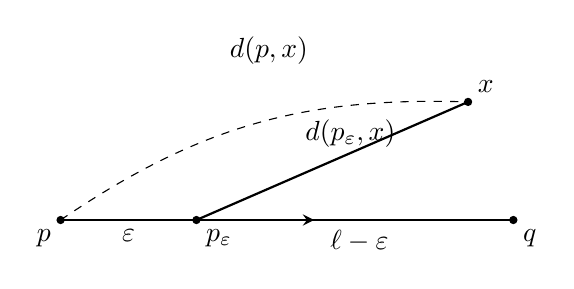
\begin{tikzpicture}[x=1.15cm,y=1cm,>=stealth]
	\coordinate (p) at (0,0);
	\coordinate (e) at (1.5,0);
	\coordinate (q) at (5,0);
	\coordinate (x) at (4.5,1.5);
	\draw[thick] (p)--(q);
	\draw[thick,->] (1.9,0)--(2.8,0);
	\draw[dashed] (p) to[bend left=18] (x);
	\draw[thick] (e)--(x);
	\node[above] at (2.3,1.85) {\(d(p,x)\)};
	\node[above,sloped] at (3.2,.8) {\(d(p_\varepsilon,x)\)};
	\node[below] at (.75,0) {\(\varepsilon\)};
	\node[below] at (3.3,0) {\(\ell-\varepsilon\)};
	\foreach \a in {p,e,q,x} {\fill (\a) circle (1.5pt);}
	\node[below left] at (p) {\(p\)};
	\node[below right] at (e) {\(p_\varepsilon\)};
	\node[below right] at (q) {\(q\)};
	\node[above right] at (x) {\(x\)};
\end{tikzpicture}

	\caption[移动基点构造距离的上支撑]{沿一条最短线把基点从 \(p\) 移到 \(p_\varepsilon\)。从 \(p\) 经 \(p_\varepsilon\) 到 \(x\) 的路线给出 \(r(x)\le\varepsilon+d(p_\varepsilon,x)\)，在 \(q\) 处取等号。图中的直线和弧线仅示意连接关系。}
	\label{g3:fig:distance-support}
\end{figure}

为准确说明“在割点仍成立”，暂记 \(L=\operatorname{div}\operatorname{grad}=-\Delta\)。若连续函数 \(f\) 在 \(q\) 附近满足：对每个 \(\eta>0\)，都有光滑函数 \(h\ge f\)，使 \(h(q)=f(q)\) 且 \(Lh(q)\le b+\eta\)，就称 \(Lf(q)\le b\) 在\term[shangzhicheng yiyi]{上支撑意义}[upper support sense]下成立，也称为相应的\term[pingzhang yiyi]{屏障意义}[barrier sense]。Hessian 的上支撑比较类似定义，以双线性型不等式 \(\operatorname{Hess}h(q)\le B+\eta g_q\) 代替迹不等式。支撑函数只需在 \(q\) 的一个邻域定义，邻域可以随 \(\eta\) 改变。

\begin{theorem}\label{g3:thm:distance-barrier-comparison}
	记 \(L=\operatorname{div}_g\operatorname{grad}_g\)、\(\Delta=-L\)，即采用非负 Laplace 算子约定。
	对给定 \(k\in\mathbb R\)，记 \(s_k\) 为满足 \(s_k''+ks_k=0\)、\(s_k(0)=0\)、\(s_k'(0)=1\) 的模型函数，\(b_k=\pi/\sqrt k\)（\(k>0\)）或 \(b_k=\infty\)（\(k\le0\)），\(\operatorname{ct}_k=s_k'/s_k\) 于 \((0,b_k)\)。
	设 \((M^n,g)\) 连通、完备、光滑且无边界，\(n\ge2\)，\(p\in M\)，\(r=d(p,\cdot)\)，\(k\in\mathbb R\)。若 \(\operatorname{Ric}\ge(n-1)kg\)，则在 \(0<r(q)<b_k\) 的每一点，包括割点，
	\[
		Lr(q)\le(n-1)\operatorname{ct}_k(r(q))
	\]
	在上支撑意义下成立；按本书符号，这就是相应的 \(\Delta r\ge-(n-1)\operatorname{ct}_k(r)\) 屏障估计。若更强地有截面曲率 \(K\ge k\)，选任一从 \(p\) 到 \(q\) 的单位速最短线的末速度 \(v\)，还得到上支撑意义下
	\[
		\operatorname{Hess}r(q)\le\operatorname{ct}_k(r(q))
		\bigl(g_q-v^\flat\otimes v^\flat\bigr).
	\]
\end{theorem}
\begin{proof}
	记 \(\ell=r(q)\)，应用上一引理。\(q\) 距新基点 \(p_\varepsilon\) 为 \(\ell-\varepsilon\)，且在其割迹之外。\cref{g3:thm:laplacian-comparison}给出
	\[
		Lr_\varepsilon(q)\le(n-1)\operatorname{ct}_k(\ell-\varepsilon).
	\]
	因为 \(0<\ell<b_k\)，右边在 \(\varepsilon\downarrow0\) 时趋于 \((n-1)\operatorname{ct}_k(\ell)\)。对给定 \(\eta>0\) 选足够小的 \(\varepsilon\)，即可得到定义要求的上支撑函数。截面曲率下界时，\cref{g3:thm:hessian-comparison}同样给出
	\[
		\operatorname{Hess}r_\varepsilon(q)
		\le\operatorname{ct}_k(\ell-\varepsilon)
		\bigl(g_q-v^\flat\otimes v^\flat\bigr).
	\]
	张量 \(g_q-v^\flat\otimes v^\flat\) 的算子范数为1，故系数的收敛也给出任意小的 \(\eta g_q\) 误差。
\end{proof}

这个构造在 \(\Delta=-L\) 的约定下仍使用距离的上支撑，而支撑函数的 \(\Delta\) 满足下界。它也给出一个便于辨认方向的测试：若光滑 \(\psi\le r\) 在 \(q\) 与 \(r\) 接触，则 \(\psi\le r_\varepsilon\) 且接触值相同，故 \(L\psi(q)\le Lr_\varepsilon(q)\)；取极限得到同一个上界。相反，截面曲率上界所给的光滑区域 Hessian 下界一般不能穿过割迹，因为割迹处的折角可能向下。

\subsection{分布意义下的 Laplace 比较}
\label{g3:subsec:0704:03}

屏障估计是逐点的接触陈述。积分论证还需要分布意义：把可能不光滑的函数与光滑紧支测试函数配对，将导数移到测试函数上。这里直接处理距离函数所需的情形。

\begin{lemma}\label{g3:lem:lipschitz-weak-gradient}
	记 \(L=\operatorname{div}_g\operatorname{grad}_g\)、\(\Delta=-L\)，即采用非负 Laplace 算子约定。
	设 \((M,g)\) 为光滑无边界黎曼流形，\(U\subset M\) 开，\(f:U\to\mathbb R\) 局部 Lipschitz，并在某个闭零测集 \(Z\) 之外光滑。则 \(f\) 的弱梯度由 \(U\setminus Z\) 上的经典梯度几乎处处给出。具体地，对任意光滑紧支向量场 \(X\) 及任意 \(\phi\in C_c^\infty(U)\)，
	\[
		\int_U f\operatorname{div}X\,\mu_g
		=-\int_U\langle\nabla f,X\rangle\,\mu_g,
		\qquad
		\int_U f\Delta\phi\,\mu_g
		=\int_U\langle\nabla f,\nabla\phi\rangle\,\mu_g.
	\]
\end{lemma}
\begin{proof}
	在相对紧坐标盒中，黎曼距离和坐标 Euclid 距离局部互相控制，因此 \(f\) 在坐标中也 Lipschitz。固定除 \(x^i\) 外的坐标，所得一元函数 Lipschitz，因而绝对连续：不交小区间上的函数增量绝对值之和至多为 Lipschitz 常数乘总长度。绝对连续函数的微积分基本定理给出该直线上的积分分部公式，其导数几乎处处存在且有界。

	由 Fubini，几乎每条坐标直线与 \(Z\) 相交于一维零测集。在其余点，刚才的一元导数等于光滑函数的 \(\partial_i f\)。再次用 Fubini，对紧支光滑 \(a\) 有
	\[
		\int f\,\partial_i a\,\mathrm{d}x
		=-\int (\partial_i f)a\,\mathrm{d}x.
	\]
	在此式中取 \(a=\sqrt{\det G}\,X^i\)，求和并使用第一章的散度坐标公式，便得坐标盒内的第一个等式。用有限个从属坐标片的光滑权重分解 \(X\)，额外的权重导数因和为1而相消，得到全局式。最后取 \(X=\nabla\phi\)，再用 \(\Delta=-\operatorname{div}\nabla\)，即得第二个等式。
\end{proof}

对局部可积的 \(f\)，定义分布 \(\Delta f\) 在测试函数 \(\phi\) 上的值为 \(\int f\Delta\phi\,\mu_g\)。若对每个非负 \(\phi\in C_c^\infty(U)\) 都有
\[
	\int_U f\Delta\phi\,\mu_g\ge\int_U b\phi\,\mu_g,
\]
就称 \(\Delta f\ge b\) 在\term[fenbu yiyi]{分布意义}[distributional sense]下成立。上一引理把这个定义转化为一阶导数的积分，因而可以用于1-Lipschitz 的距离函数。非负测试函数和不等式方向都是定义的一部分。

\begin{theorem}\label{g3:thm:distributional-laplacian-comparison}
	记 \(L=\operatorname{div}_g\operatorname{grad}_g\)、\(\Delta=-L\)，即采用非负 Laplace 算子约定。
	对给定 \(k\in\mathbb R\)，记 \(s_k\) 为满足 \(s_k''+ks_k=0\)、\(s_k(0)=0\)、\(s_k'(0)=1\) 的模型函数，\(b_k=\pi/\sqrt k\)（\(k>0\)）或 \(b_k=\infty\)（\(k\le0\)），\(\operatorname{ct}_k=s_k'/s_k\) 于 \((0,b_k)\)。
	设 \((M^n,g)\) 连通、完备、光滑且无边界，\(n\ge2\)，\(\operatorname{Ric}\ge(n-1)kg\)，\(p\in M\)。令 \(r=d(p,\cdot)\)、\(U_k=\{x:0<r(x)<b_k\}\)。则在 \(U_k\) 上
	\begin{equation}\label{g3:eq:distributional-laplacian-comparison}
		\Delta r\ge-(n-1)\operatorname{ct}_k(r)
	\end{equation}
	在分布意义下成立。等价地，对每个非负 \(\phi\in C_c^\infty(U_k)\)，
	\[
		\int_{U_k}\langle\nabla r,\nabla\phi\rangle\,\mu_g
		\ge-\int_{U_k}(n-1)\operatorname{ct}_k(r)\phi\,\mu_g.
	\]
\end{theorem}
\begin{proof}
	距离为1-Lipschitz，且在闭零测集 \(\{p\}\cup\operatorname{Cut}(p)\) 外光滑，故上一引理适用。取 \(0<a<R<b_k\)，使 \(\phi\) 的支集包含于 \(\{a<r<R\}\)，并把 \(R\) 取得严格大于支集上的最大距离。在式\eqref{g3:eq:polar-cut-integration}中写
	\[
		\Phi(t,u)=\phi(\exp_p(tu)),\qquad
		\tau(u)=\min\{c_p(u),R\}.
	\]
	当 \(0<t<c_p(u)\) 时，\(\nabla r=\partial_t\)，所以
	\[
		\int\langle\nabla r,\nabla\phi\rangle\,\mu_g
		=\int_{S_pM}\int_0^{\tau(u)}\partial_t\Phi\,\theta\,\mathrm{d}t\,\mathrm{d}\sigma(u).
	\]
	对每条射线作一元分部积分。起端项为零，因为 \(\Phi=0\) 于支集以前；末端在 \(\tau=R\) 时同样为零，在有限割时 \(\tau=c_p(u)<R\) 时为
	\(\Phi(c_p(u),u)\theta(c_p(u),u)\ge0\)。这里 \(A_u\) 光滑延拓至割时，\(\theta\) 从正值趋于非负值；若该端点共轭，行列式就是零。因此
	\begin{equation}\label{g3:eq:cut-boundary-flux}
		\int\langle\nabla r,\nabla\phi\rangle\,\mu_g
		=\mathcal B_p(\phi)-\int_{S_pM}\int_0^{\tau(u)}\Phi\,\partial_t\theta\,\mathrm{d}t\,\mathrm{d}\sigma,
		\qquad \mathcal B_p(\phi)\ge0.
	\end{equation}
	这些积分和端点极限可以按方向积分：在紧集 \(S_pM\times[0,R]\) 上，Jacobi 方程的光滑依赖给出 \(\theta\)、\(\partial_t\theta\) 的共同界，而 \(c_p\) 可测，测试函数又有紧支集。

	在割时之前，由\cref{g3:thm:riccati-trace-comparison}和行列式求导，
	\[
		\partial_t\theta=h\theta
		\le(n-1)\operatorname{ct}_k(t)\theta.
	\]
	由于 \(\Phi\ge0\)，将此式代入 \eqref{g3:eq:cut-boundary-flux}并保留非负末端项，得到
	\[
		\int\langle\nabla r,\nabla\phi\rangle\,\mu_g
		\ge-\int_{S_pM}\int_0^{\tau(u)}
		(n-1)\operatorname{ct}_k(t)\Phi\theta\,\mathrm{d}t\,\mathrm{d}\sigma.
	\]
	再用极坐标换元，右端就是所要求的积分。这个证明同时说明：割迹的贡献在 \(Lr\) 中为非正，在本书的 \(\Delta r\) 中为非负。
\end{proof}

常曲率的逐点公式不能照搬为越过割迹的分布等式。例如平坦圆柱上，距离在一条割线上由两支光滑函数取较小者；两支的一阶导数在那里发生向下跳跃。因此即使所有光滑点都满足模型等式，分布中仍会多出割线项。章末习题将计算这一项。

\subsection{等号传播及局部空间形式}
\label{g3:subsec:0704:04}

比较中的等号记录了证明里各个非负量同时消失。Rauch 比较的单一方向等号控制一条 Jacobi 场；Ricci 迹比较的等号还使径向形算子各特征值相同。只有在一族方向上获得这些信息，才会确定一个开区域的度量。

\begin{proposition}\label{g3:prop:radial-metric-evolution}
	将法向空间沿线平行识别，径向 Jacobi 张量 \(A\) 满足 \(A''+\mathcal RA=0\)、\(A(0)=0\)、\(A'(0)=I\)，其中 \(\mathcal R=R(\cdot,\dot\gamma)\dot\gamma\)；在 \(A\) 可逆处记 \(S=A'A^{-1}\)、\(h=\operatorname{tr}S\)，\(I\) 为恒等算子。
	沿所述测地线，\(T=\dot\gamma\)，\(R\) 表示 Levi-Civita 曲率，\(P\) 表示沿线平行移动，撇号表示协变导数。
	对给定 \(k\in\mathbb R\)，记 \(s_k\) 为满足 \(s_k''+ks_k=0\)、\(s_k(0)=0\)、\(s_k'(0)=1\) 的模型函数，\(b_k=\pi/\sqrt k\)（\(k>0\)）或 \(b_k=\infty\)（\(k\le0\)），\(\operatorname{ct}_k=s_k'/s_k\) 于 \((0,b_k)\)。
	设 \((M^n,g)\) 为光滑无边界黎曼流形，\(p\in M\)，且 \(\exp_p\) 在切球 \(B_R(0)\) 上为微分同胚。令 \(F(t,u)=\exp_p(tu)\)，\(0<t<R\)、\(u\in S_pM\)。则
	\[
		F^*g=\mathrm{d}t^2+G_t,
	\]
	其中 \(G_t\) 是单位切球面上的度量族。若沿每条射线有 \(S(t)=\operatorname{ct}_k(t)I\)，且 \(R\le b_k\)，则
	\begin{equation}\label{g3:eq:model-polar-metric-rigidity}
		G_t=s_k(t)^2g_{S_pM}.
	\end{equation}
\end{proposition}
\begin{proof}
	Gauss 引理给出径向与角向的正交分解。对 \(u^\perp=\mathrm{T}_uS_pM\) 中的 \(a,b\)，令 \(J_a,J_b\) 为对应角向 Jacobi 场，则
	\[
		G_t(a,b)=\langle J_a(t),J_b(t)\rangle.
	\]
	径向形算子满足 \(J_a'=SJ_a\)，故
	\[
		\partial_tG_t(a,b)
		=\langle SJ_a,J_b\rangle+\langle J_a,SJ_b\rangle.
	\]
	当 \(S=\operatorname{ct}_k I\) 时，右端为 \(2\operatorname{ct}_kG_t(a,b)\)，于是 \(\partial_t(s_k^{-2}G_t)=0\)。另一方面，\(J_a(t)=tP_ta+O(t^3)\)、\(s_k(t)/t\to1\)，因此 \(s_k(t)^{-2}G_t(a,b)\to\langle a,b\rangle\)。常数只能是单位切球面的标准度量，得到式\eqref{g3:eq:model-polar-metric-rigidity}。
\end{proof}

\begin{theorem}\label{g3:thm:laplacian-equality-local-space-form}
	记 \(L=\operatorname{div}_g\operatorname{grad}_g\)、\(\Delta=-L\)，即采用非负 Laplace 算子约定。
	对给定 \(k\in\mathbb R\)，记 \(s_k\) 为满足 \(s_k''+ks_k=0\)、\(s_k(0)=0\)、\(s_k'(0)=1\) 的模型函数，\(b_k=\pi/\sqrt k\)（\(k>0\)）或 \(b_k=\infty\)（\(k\le0\)），\(\operatorname{ct}_k=s_k'/s_k\) 于 \((0,b_k)\)。
	设 \((M^n,g)\) 连通、完备、光滑且无边界，\(n\ge2\)，\(\operatorname{Ric}\ge(n-1)kg\)，\(p\in M\)，\(r=d(p,\cdot)\)。设 \(0<R<\min\{\operatorname{inj}_g(p),b_k\}\)。若对每个 \(u\in S_pM\)，在 \(q=\exp_p(Ru)\) 处都有
	\[
		\Delta r(q)=-(n-1)\operatorname{ct}_k(R),
	\]
	则 \(B(p,R)\) 与常截面曲率 \(k\) 的标准模型中半径 \(R\) 的球等距，且等距可取为指定起点切空间线性等距所诱导的指数坐标对应。
\end{theorem}
\begin{proof}
	沿任意固定方向 \(u\)，所给等号就是 \(h(R)=(n-1)\operatorname{ct}_k(R)\)。由\cref{g3:prop:riccati-trace-rigidity}，该方向上全部 \(0<t\le R\) 满足 \(S=\operatorname{ct}_k I\)。其证明中的等号分别使 \(\operatorname{Ric}(T,T)=(n-1)k\) 和无迹部分 \(S-hI/(n-1)\) 为零；因此得到的是整个径向算子的结论。对所有方向应用上一命题，便有
	\[
		F^*g=\mathrm{d}t^2+s_k(t)^2g_{S_pM}.
	\]
	在标准常曲率模型上，\cref{g3:exm:constant-curvature-jacobi}给出同样的角向 Jacobi 场和同样的极坐标度量。任选两起点切空间间的线性等距，先在切球中对应向量，再分别使用指数映射，就得到穿孔球上的等距。该对应本身在中心光滑，其微分为所选线性等距，所以由度量的连续性，中心处也保持度量。\(R\) 小于两侧的指数单射半径，故该对应是整个球的微分同胚与等距。
\end{proof}

这里只需在整张半径 \(R\) 的测地球面上取得迹等号，就能沿各射线向内恢复整个球的度量。若只在一个方向取得等号，结论相应限于这一条射线；若只知道一支 Jacobi 场的长度达到 Rauch 等号，控制的方向还要更少。下一章将把径向密度的不等式沿方向积分，得到球体积比较，并继续分析整体几何受到的限制。
% 纲要条目排为编号小节标题，并进入目录与书签；说明段仍保留于纲要注释中。


\begin{chaptersummary}
	指标形式的端点极小性给出曲率与径向伸缩的比较，积分后便是 Rauch 长度估计。较大的截面曲率使共同初始导数的法向 Jacobi 场受到更强的约束；比较必须在模型函数为正并满足所需非共轭条件的区间内进行。指数映射微分的估计是局部长度信息，不能单独保证全局单射或最短性。

	\ProseParagraphBreak

	矩阵 \(S=A'A^{-1}\) 同时描述 Jacobi 场的相对增长和测地球面的径向变化。Riccati 方程取迹后，\(\operatorname{tr}S^2\ge(\operatorname{tr}S)^2/(n-1)\) 把 Ricci 下界变为迹上界；无迹部分是否消失决定了等号。距离 Hessian 是这个算子的几何表达，极坐标密度的对数导数则是它的迹。

	\ProseParagraphBreak

	割迹外的光滑比较可用移动基点延伸为上支撑估计，也可用极坐标分部积分延伸为分布不等式；后者保留了割点处符号确定的边界贡献。等号先沿射线向内传播，若整张测地球面的迹都达到模型值，就能恢复球内的极坐标度量。下一章将进一步沿方向和半径积分，研究体积、直径与整体拓扑约束。
\end{chaptersummary}

\BookExercises

\begin{exercise}\label{g3:ex:rauch-equality-single-geodesic}
	在 \(M=\mathbb R\times S^2(a)\) 上取乘积度量，固定 \(p=(0,q)\)，令 \(u\) 为实直线因子的正向单位向量，\(\gamma(t)=(t,q)\)。
	\begin{enumerate}
		\item 证明 \(M\) 的截面曲率非负，但沿 \(\gamma\) 的每个径向截面曲率都为零。
		\item 求沿 \(\gamma\) 满足 \(J(0)=0\) 的所有 Jacobi 场，并证明对每个 \(t>0\)，\((\mathrm d\exp_p)_{tu}\) 都是线性等距。
		\item 证明 \(\gamma\) 的任一点都没有与 Euclid 空间局部等距的邻域。由此说明，在一条固定的径向测地线上，所有初始法向方向都达到 Rauch 平坦模型的等号，仍不足以确定邻域的度量。
	\end{enumerate}
\end{exercise}
\begin{solution}
	设 \(X=(x,X_S)\)、\(Y=(y,Y_S)\) 为乘积中的切向量。由\cref{g3:prop:product-curvature}，
	\[
		\langle R(X,Y)Y,X\rangle
		=\frac1{a^2}\bigl(|X_S|^2|Y_S|^2-\langle X_S,Y_S\rangle^2\bigr)\ge0.
	\]
	若 \(X=u\)，其球面分量为零，曲率分子为零；故含 \(u\) 的每个截面曲率均为零。事实上，乘积曲率公式还给出 \(R(V,u)u=0\) 对任意 \(V\) 成立。

	于是沿 \(\gamma\) 的 Jacobi 方程为 \(J''=0\)。若 \(P_t\) 为从 \(0\) 到 \(t\) 的平行移动，所有初始值为零的解恰为
	\[
		J_w(t)=tP_tw,\qquad w\in \mathrm{T}_pM.
	\]
	由指数映射的微分公式，
	\[
		(\mathrm d\exp_p)_{tu}(w)=\frac1tJ_w(t)=P_tw,
	\]
	所以微分是线性等距。这也说明沿该线无共轭时刻。

	另一方面，每点的球面因子切平面都有截面曲率 \(a^{-2}>0\)。局部等距保持曲率，而 Euclid 空间所有截面曲率为零，因此任一点附近都不可能与 Euclid 空间局部等距。该例在固定的一条径向线上取等号，却没有在从 \(p\) 出发的一个开集方向上给出同样信息；邻域刚性需要这样的额外方向条件。
\end{solution}

\begin{exercise}\label{g3:ex:normal-coordinate-bilipschitz}
	设 \((M,g)\) 为光滑无边界黎曼流形，\(p\in M\)，\(\kappa>0\)，且 \(0<\rho<\pi/\sqrt\kappa\)。假设 \(\exp_p\) 把切空间开球 \(B(0,\rho)\) 微分同胚地映到 \(U\)，并且每条从 \(p\) 出发、参数小于 \(\rho\) 的径向测地线上的径向截面曲率都满足 \(-\kappa\le K\le\kappa\)。令
	\[
		\alpha=\frac{\sin(\sqrt\kappa\,\rho)}{\sqrt\kappa\,\rho},
		\qquad
		\beta=\frac{\sinh(\sqrt\kappa\,\rho)}{\sqrt\kappa\,\rho}.
	\]
	证明法坐标中的拉回度量满足
	\[
		\alpha^2|\xi|^2
		\le (\exp_p^*g)_v(\xi,\xi)
		\le\beta^2|\xi|^2
		\qquad(v\in B(0,\rho),\ \xi\in \mathrm{T}_pM).
	\]
	记 \(d_U\) 为只允许曲线留在 \(U\) 内所定义的路径距离。进一步证明
	\[
		\alpha|v-w|
		\le d_U(\exp_pv,\exp_pw)
		\le\beta|v-w|.
	\]
	说明为何一般不能直接把中间的 \(d_U\) 换成 \(M\) 的距离，以及强凸性为何足以允许这种替换。
\end{exercise}
\begin{solution}
	设 \(v=ru\ne0\)、\(|u|=1\)，写 \(\xi=bu+z\)、\(z\perp u\)。由\cref{g3:prop:exponential-length-comparison}的双边形式，
	\[
		b^2+\left(\frac{s_\kappa(r)}r\right)^2|z|^2
		\le(\exp_p^*g)_v(\xi,\xi)
		\le b^2+\left(\frac{s_{-\kappa}(r)}r\right)^2|z|^2.
	\]
	其中曲率上界先保证 \(r<\pi/\sqrt\kappa\) 时没有共轭点，故两个方向均可用。

	为取得整个坐标球上的常数，注意
	\[
		\frac{\mathrm d}{\mathrm dr}\frac{s_k(r)}r
		=\frac1{r^2}\int_0^r\bigl(c_k(r)-c_k(t)\bigr)\,\mathrm dt.
	\]
	在 \((0,\pi/\sqrt\kappa)\) 上，\(c_\kappa(t)=\cos(\sqrt\kappa\,t)\) 递减，故 \(s_\kappa(r)/r\) 递减；\(c_{-\kappa}(t)=\cosh(\sqrt\kappa\,t)\) 递增，故 \(s_{-\kappa}(r)/r\) 递增。二者在 \(0\) 的极限都为 \(1\)，因而
	\[
		0<\alpha\le\frac{s_\kappa(r)}r\le1
		\le\frac{s_{-\kappa}(r)}r\le\beta.
	\]
	代入即可得到度量估计，在 \(v=0\) 处由 \((\mathrm d\exp_p)_0=I\) 成立。

	任取 \(U\) 中连接 \(\exp_pv\) 与 \(\exp_pw\) 的分段光滑曲线，拉回为球中的曲线 \(c\)，度量下界给出
	\[
		\operatorname{Len}_g(\exp_p\circ c)
		\ge\alpha\operatorname{Len}_{g_p}(c)
		\ge\alpha|v-w|.
	\]
	取下确界得到距离下界。为得上界，用切空间中的直线段连接 \(v,w\)；开球凸，所以整段仍在球内。度量上界给出其像的长度至多为 \(\beta|v-w|\)。

	流形距离允许连接曲线离开 \(U\)，因此一般只有 \(d_M\le d_U\)，上述下界不能自动传给 \(d_M\)。如果 \(U\) 强凸，每对点之间的全局最短测地线都留在 \(U\)，故 \(d_M=d_U\)，两边的估计便同时成立。
\end{solution}

\begin{exercise}\label{g3:ex:first-conjugate-upper-bound-rigidity}
	取 \(k\in\mathbb R\)。记 \(s_k\) 为 \(s_k''+ks_k=0\)、\(s_k(0)=0\)、\(s_k'(0)=1\) 的解，\(c_k=s_k'\)、\(\operatorname{ct}_k=c_k/s_k\)，\(b_k=\pi/\sqrt k\) 当 \(k>0\)，否则 \(b_k=\infty\)。
	设 \(\gamma:[0,b_k]\to M\) 是 \(n\ge2\) 维光滑无边界黎曼流形中的单位速测地线，延拓到端点邻域，其中 \(k>0\)、\(b_k=\pi/\sqrt k\)。假设沿线每个径向截面满足 \(K\ge k\)。证明以下两项等价：
	\begin{enumerate}
		\item 相对起点的第一个正共轭时刻恰为 \(b_k\)。
		\item 在 \(0\le t\le b_k\) 上，对所有 \(V\perp\dot\gamma(t)\) 都有 \(R(V,\dot\gamma)\dot\gamma=kV\)。
	\end{enumerate}
	证明此时 \(b_k\) 处的共轭重数为 \(n-1\)。进一步说明，若某个内时刻存在径向截面曲率严格大于 \(k\)，则首共轭时刻必严格小于 \(b_k\)。提示：使用首个共轭端点处指标形式的半正定性，以及两端为零的模型试探场。
\end{exercise}
\begin{solution}
	先假设第一个正共轭时刻为 \(b_k\)。取任意平行单位法向场 \(E\)，令 \(V(t)=s_k(t)E(t)\)。由于 \(s_k(0)=s_k(b_k)=0\)，场 \(V\) 两端为零。\cref{g3:prop:first-conjugate-semidefinite}给出 \(I_\gamma(V)\ge0\)，而曲率下界给出
	\[
		I_\gamma(V)\le I_k(V)
		=\int_0^{b_k}\bigl((s_k')^2-ks_k^2\bigr)\,\mathrm dt
		=[s_ks_k']_0^{b_k}=0.
	\]
	因此两个指标值都为零，且
	\[
		0=I_k(V)-I_\gamma(V)
		=\int_0^{b_k}s_k(t)^2
		\bigl(\langle R(E,T)T,E\rangle-k\bigr)\,\mathrm dt.
	\]
	被积函数连续、非负，而 \(s_k>0\) 于内部，故 \(\langle R(E,T)T,E\rangle=k\) 在整个内部成立，在端点由连续性成立。任一时刻的任意单位法向量都可平行延拓成这样的 \(E\)，所以曲率算子的二次型在法空间上恒为 \(k|V|^2\)。算子自伴，由极化便得到 \(R(V,T)T=kV\)。

	反过来，若第二项成立，所有法向零初值 Jacobi 场都为
	\[
		J_w(t)=s_k(t)P_{t\leftarrow0}w,
		\qquad w\perp T(0).
	\]
	它们在 \(0<t<b_k\) 处没有非零场消失，在 \(b_k\) 处则全部消失。切向零初值解为 \(atT\)，在正时刻不能再次消失，除非 \(a=0\)。因此首共轭时刻正是 \(b_k\)，重数为法空间维数 \(n-1\)。

	最后，\cref{g3:prop:conjugate-radius-comparison}已经保证首共轭时刻不超过 \(b_k\)。若在某个内时刻有径向截面曲率严格大于 \(k\)，第二项不成立，刚证的等价性排除首时刻等于 \(b_k\)，故必严格小于 \(b_k\)。
\end{solution}

\begin{exercise}\label{g3:ex:riccati-higher-radial-expansion}
	设 \((M^n,g)\) 为光滑无边界黎曼流形，\(n\ge2\)，\(\gamma(t)=\exp_p(tv)\) 为单位速测地线，\(m=n-1\)。记 \(\mathcal R=R(\cdot,\dot\gamma)\dot\gamma\) 为法向曲率算子，\(A\) 为满足 \(A(0)=0,A'(0)=I\) 的径向 Jacobi 张量，\(S=A'A^{-1}\)、\(\theta=\det A\)。在沿线平行标架中记 \(\mathcal R_0=\mathcal R(0)\)、\(\mathcal R_1=\mathcal R'(0)\)。将式\eqref{g3:eq:radial-riccati-initial}再展开一阶，求 \(A(t)\) 的四次项、\(S(t)\) 的二次项以及 \(\theta(t)/t^m\) 的三次项。说明把初始方向 \(v\) 改为 \(-v\) 时，最后一个三次项怎样变化。
\end{exercise}
\begin{solution}
	对 \(A''=-\mathcal R A\) 连续求导并在零处代入 \(A(0)=0\)、\(A'(0)=\operatorname{id}\)，得到
	\[
		A''(0)=0,\qquad A'''(0)=-\mathcal R_0,\qquad A^{(4)}(0)=-2\mathcal R_1.
	\]
	所以光滑性和 Taylor 定理给出
	\[
		\begin{aligned}
		A(t)&=t\operatorname{id}-\frac{t^3}{6}\mathcal R_0-\frac{t^4}{12}\mathcal R_1+O(t^5),\\
		A'(t)&=\operatorname{id}-\frac{t^2}{2}\mathcal R_0-\frac{t^3}{3}\mathcal R_1+O(t^4),\\
		A(t)^{-1}&=t^{-1}\left(\operatorname{id}+\frac{t^2}{6}\mathcal R_0+\frac{t^3}{12}\mathcal R_1+O(t^4)\right).
		\end{aligned}
	\]
	将后两式相乘，二次以上的小矩阵相互乘积只影响 \(S\) 的三次及更高次项，故
	\[
		S(t)=t^{-1}\operatorname{id}-\frac t3\mathcal R_0-\frac{t^2}{4}\mathcal R_1+O(t^3).
	\]
	另一方面，\(\det(\operatorname{id}+X)=1+\operatorname{tr}X+O(\lVert X\rVert^2)\)，且此处 \(X=O(t^2)\)。因此
	\[
		\frac{\theta(t)}{t^m}
		=1-\frac{t^2}{6}\operatorname{Ric}_p(v,v)
		-\frac{t^3}{12}(\nabla_v\operatorname{Ric})_p(v,v)+O(t^4).
	\]
	迹与沿线协变导数可交换，而 \(v\) 沿测地线平行，这说明 \(\operatorname{tr}\mathcal R_1=(\nabla_v\operatorname{Ric})(v,v)\)。反向射线的 \(\operatorname{Ric}_p(-v,-v)=\operatorname{Ric}_p(v,v)\)，但
	\((\nabla_{-v}\operatorname{Ric})_p(-v,-v)=-(\nabla_v\operatorname{Ric})_p(v,v)\)，故二次项不变、三次项变号。点处密度在相反方向的首个可能差异出现在这一奇次项。
\end{solution}

\begin{exercise}\label{g3:ex:product-strict-trace-comparison}
	在乘积 \(M=\mathbb H^2(-a^2)\times\mathbb R\) 上取乘积度量，其中 \(a>0\)，第一因子的常曲率为 \(-a^2\)。设单位速测地线 \(\gamma\) 完全沿第一因子行走。求它的法向径向 Jacobi 张量 \(A\)、\(S=A'A^{-1}\)、\(h=\operatorname{tr}S\) 和密度 \(\theta=\det A\)。用迹比较说明，对每个 \(t>0\)，
	\[
		a\coth(at)+\frac1t<\sqrt2\,a\coth\left(\frac{at}{\sqrt2}\right),
		\qquad
		\frac{t\sinh(at)}a<\frac2{a^2}\sinh^2\left(\frac{at}{\sqrt2}\right).
	\]
	解释为什么沿线 \(\operatorname{Ric}(T,T)\) 恰好等于模型下界，比较却仍严格。
\end{exercise}
\begin{solution}
	取第一因子中与 \(T\) 垂直的平行单位场 \(E_1\)，以及第二因子的单位场 \(E_2\)。\cref{g3:prop:product-curvature}的乘积曲率公式给出
	\(\mathcal R=\operatorname{diag}(-a^2,0)\)。分别解两个标量 Jacobi 初值问题，得到
	\[
		A(t)=\begin{pmatrix}\sinh(at)/a&0\\0&t\end{pmatrix},\qquad
		S(t)=\begin{pmatrix}a\coth(at)&0\\0&1/t\end{pmatrix}.
	\]
	于是
	\[
		h(t)=a\coth(at)+\frac1t,\qquad
		\theta(t)=\frac{t\sinh(at)}a.
	\]
	两项分离量对 \(t>0\) 都不为零，故不存在正共轭时刻。这里 \(m=2\)、\(\operatorname{Ric}(T,T)=-a^2=mk\)，应选 \(k=-a^2/2\)。模型迹与密度正是题设两个右端，\cref{g3:thm:riccati-trace-comparison,g3:prop:radial-density-comparison}给出不严格比较。

	对 \(x>0\)，函数 \(x\cosh x-\sinh x\) 在零处为零，导数为 \(x\sinh x>0\)。因此 \(x\coth x>1\)，从而 \(S\) 的两个特征值始终不相等。式\eqref{g3:eq:riccati-trace-cauchy-schwarz}的差值严格为正。尽管 Ricci 误差项为零，式\eqref{g3:eq:riccati-trace-defect}中的 \(F\) 仍处处为正，故迹比较严格。密度比的对数导数严格为负，且比值在起点趋于一，所以密度比较也严格。这个例子显示，Ricci 等于模型值并不保证各个方向的扩张率相同。
\end{solution}

\begin{exercise}\label{g3:ex:regular-riccati-focusing}
	设 \(m\ge1\)，\(\mathcal R(t)\) 是定义于 \([0,\infty)\) 的光滑实对称 \(m\) 阶矩阵函数，且 \(\operatorname{tr}\mathcal R(t)\ge0\)。设实对称矩阵解 \(S\) 满足
	\[
		S'+S^2+\mathcal R=0,\qquad \operatorname{tr}S(0)=-\alpha<0.
	\]
	证明：\(S\) 不能作为有限光滑矩阵解存在到时刻 \(m/\alpha\)。说明这与径向解在零处的奇异初值问题有何不同，并给出达到这一时间上界的 Euclid 法线聚焦模型。
\end{exercise}
\begin{solution}
	令 \(h=\operatorname{tr}S\)。迹方程与 Cauchy--Schwarz 不等式给出
	\[
		h'=-\operatorname{tr}(S^2)-\operatorname{tr}\mathcal R
		\le-\frac{h^2}{m}.
	\]
	因此 \(h\) 不增，始终不大于 \(-\alpha\)，可以取倒数。对存在区间内的每个 \(t\ge0\)，有
	\[
		\left(\frac1h\right)'=-\frac{h'}{h^2}\ge\frac1m,
		\qquad
		\frac1{h(t)}\ge-\frac1\alpha+\frac tm.
	\]
	若有限矩阵解存在到 \(t=m/\alpha\)，右端非负，而左端严格为负，矛盾。对 \(0\le t<m/\alpha\) 还可写为
	\[
		h(t)\le-\frac{\alpha}{1-\alpha t/m}.
	\]
	为解释有限端点处的发散，取线性系统 \(A''+\mathcal R A=0\)、\(A(0)=\operatorname{id}\)、\(A'(0)=S(0)\) 的全区间解；其存在性由\cref{g3:thm:jacobi-initial-data}证明中的线性系统方法得到。在 \(S\) 的存在区间内，令 \(Z=A'-SA\)，则 \(Z'=-SZ\)、\(Z(0)=0\)，故 \(A'=SA\) 且 \(\det A(t)=\exp(\int_0^t h)\)。若最大存在区间右端 \(\tau\) 有限而 \(S\) 有界，则该行列式在 \(\tau\) 仍有正的极限，所以 \(A'A^{-1}\) 在 \(\tau\) 附近光滑并延拓 \(S\)，矛盾。因此有限端点确实伴随矩阵失去有界性。

	令 \(b=m/\alpha\)，取 \(\mathcal R=0\)、\(S(t)=-(b-t)^{-1}\operatorname{id}\)，则方程成立，初始迹为 \(-m/b=-\alpha\)，并恰在 \(b\) 处爆破。它是 \(\mathbb R^{m+1}\) 中半径 \(b\) 球面的内法线族：沿法线的切向分离张量为
	\(A(t)=(1-t/b)\operatorname{id}\)，在球心同时消失。这里初始截面是一个具有有限形算子的超曲面，\(S(0)=-b^{-1}\operatorname{id}\) 有限；从单点发出的径向族则有 \(A(0)=0\)、\(S(t)\sim t^{-1}\operatorname{id}\)，不能把本题的有限初值直接放到那个奇异起点上。
\end{solution}

\begin{exercise}\label{g3:ex:model-radial-potential}
	取 \(k\in\mathbb R\)。记 \(s_k\) 为 \(s_k''+ks_k=0\)、\(s_k(0)=0\)、\(s_k'(0)=1\) 的解，\(c_k=s_k'\)、\(\operatorname{ct}_k=c_k/s_k\)，\(b_k=\pi/\sqrt k\) 当 \(k>0\)，否则 \(b_k=\infty\)。
	设 \((M^n,g)\) 为光滑无边界黎曼流形，\(p\in M\)，\(r=d(p,\cdot)\)，\(c_p\) 为割时函数，\(T\) 为单位径向速度。定义
	\[
		\Phi_k(t)=\int_0^t s_k(u)\,\mathrm du.
	\]
	求 \(\Phi_k\) 的显式表达式，证明对任意黎曼流形的局部距离函数 \(r=d(p,\cdot)\)，\(\Phi_k(r)\) 在初点 \(p\) 光滑，且
	\(\operatorname{Hess}\Phi_k(r)|_p=g_p\)。
	在 \(0<r<\min\{c_p(u),b_k\}\) 上，分别从径向截面上界 \(K\le k\)、下界 \(K\ge k\) 推出它的 Hessian 比较；再从径向 Ricci 下界 \(\operatorname{Ric}(T,T)\ge(n-1)k\) 推出本书符号下的 Laplace 比较，并核对常曲率模型中的等号。
\end{exercise}
\begin{solution}
	积分得到
	\[
		\Phi_k(t)=
		\begin{cases}
			(1-\cos(\sqrt{k}t))/k,&k>0,\\
			t^2/2,&k=0,\\
			(\cosh(\sqrt{-k}t)-1)/(-k),&k<0.
		\end{cases}
	\]
	三个表达式在零附近都有收敛的偶次幂展开
	\[
		\Phi_k(t)=\frac{t^2}{2}-\frac{kt^4}{24}+O(t^6).
	\]
	在法坐标中 \(r^2=\sum_i(x^i)^2\)，因此把该收敛级数写成 \(r^2\) 的光滑函数，就得到初点处的光滑性；二次项给出中心 Hessian 为 \(g_p\)。

	因为 \(\Phi_k'=s_k\)、\(\Phi_k''=c_k\)，链式公式给出
	\[
		\operatorname{Hess}\Phi_k(r)
		=c_k(r)\,\mathrm dr\otimes\mathrm dr
		+s_k(r)\operatorname{Hess}r.
	\]
	在 \(0<r<b_k\) 中 \(s_k(r)>0\)，故截面上界给出
	\[
		\operatorname{Hess}\Phi_k(r)
		\ge c_k(r)\,\mathrm dr\otimes\mathrm dr+
		s_k(r)\operatorname{ct}_k(r)
		\bigl(g-\mathrm dr\otimes\mathrm dr\bigr)
		=c_k(r)g.
	\]
	截面下界给出反向不等式。这里乘以的是正数 \(s_k\)，即使 \(k>0\) 且 \(c_k\) 已变负，不等号方向也不改变。

	在 Ricci 下界下，由 \(\Phi_k'=s_k>0\) 得
	\[
		\Delta\Phi_k(r)
		\ge-c_k(r)-(n-1)s_k(r)\operatorname{ct}_k(r)
		=-n c_k(r).
	\]
	常曲率模型中 \(\operatorname{Hess}r=\operatorname{ct}_k(r)(g-\mathrm dr\otimes\mathrm dr)\)，所以
	\(\operatorname{Hess}\Phi_k(r)=c_k(r)g\)、
	\(\Delta\Phi_k(r)=-n c_k(r)\)。
	在初点 \(c_k(0)=1\)，所有公式与中心 Hessian 及 \(\Delta\Phi_k(r)(p)=-n\) 相容。
\end{solution}

\begin{exercise}\label{g3:ex:model-radial-harmonic-comparison}
	取 \(k\in\mathbb R\)。记 \(s_k\) 为 \(s_k''+ks_k=0\)、\(s_k(0)=0\)、\(s_k'(0)=1\) 的解，\(c_k=s_k'\)、\(\operatorname{ct}_k=c_k/s_k\)，\(b_k=\pi/\sqrt k\) 当 \(k>0\)，否则 \(b_k=\infty\)。
	设 \((M^n,g)\) 为光滑无边界黎曼流形，\(p\in M\)，\(r=d(p,\cdot)\)，\(T\) 为单位径向速度，\(\Delta=-\operatorname{div}_g\operatorname{grad}_g\)，\(n\ge2\)、\(0<R<b_k\)，在 \(0<t\le R\) 上定义
	\[
		G_{k,R}(t)=\int_t^R s_k(u)^{-(n-1)}\,\mathrm du.
	\]
	证明在常曲率 \(k\) 的模型中，\(G_{k,R}(r)\) 在相应穿孔球内调和。若一般流形沿从 \(p\) 出发的有关最短径向线满足
	\(\operatorname{Ric}(T,T)\ge(n-1)k\)，证明在
	\(0<r<R\) 且未到割点的范围内，
	\[
		\Delta G_{k,R}(r)\le0.
	\]
	写出 \(k=0\) 时 \(n=2\) 与 \(n>2\) 的表达式，并解释为何这里的不等号与 \(\Delta r\) 的比较方向不同。
\end{exercise}
\begin{solution}
	记 \(m=n-1\)。有
	\[
		G_{k,R}'(t)=-s_k(t)^{-m},\qquad
		G_{k,R}''(t)
		=m\operatorname{ct}_k(t)s_k(t)^{-m}
		=-m\operatorname{ct}_k(t)G_{k,R}'(t).
	\]
	因此它满足模型径向调和方程
	\(G''+m\operatorname{ct}_kG'=0\)。
	模型中 \(Lr=m\operatorname{ct}_k(r)\)，代入径向 Laplace 公式得到 \(\Delta G(r)=0\)。

	一般情形中直接保留导数的符号计算：
	\[
		\Delta G(r)
		=-G''(r)-G'(r)Lr
		=-G'(r)\bigl(Lr-m\operatorname{ct}_k(r)\bigr).
	\]
	由 Ricci 比较，括号不大于零；而 \(-G'>0\)，所以右边不大于零。等价地，这是\cref{g3:prop:radial-function-laplacian}中递减径向函数所用的方向。

	当 \(k=0\) 时，
	\[
		G_{0,R}(t)=
		\begin{cases}
			\log(R/t),&n=2,\\
			\bigl(t^{2-n}-R^{2-n}\bigr)/(n-2),&n>2.
		\end{cases}
	\]
	这些函数都递减，而 \(t\mapsto t\) 递增；链式公式中的系数 \(-f'\) 因而相反。上述调和与比较均在穿孔光滑区域内逐点成立。
\end{solution}

\begin{exercise}\label{g3:ex:ricci-bound-not-hessian-bound}
	以 \(L=\operatorname{div}_g\operatorname{grad}_g\) 记正号迹算子。利用第三章的曲率局部实现命题，构造 \(\mathbb R^3\) 上一个完备光滑度量 \(g\)，使原点附近 \(\operatorname{Ric}>0\)，但从原点沿某条单位速测地线 \(\gamma\) 出发时，存在平行单位法向场 \(E\)，对所有充分小的 \(t>0\) 满足
	\[
		\operatorname{Hess}r_{\gamma(t)}(E(t),E(t))>\frac1t,
		\qquad r=d_g(0,\cdot).
	\]
	同时证明对这些充分小的正数仍有 \(Lr\le2/t\)。说明这排除了从径向 Ricci 非负直接推出
	\(\operatorname{Hess}r\le r^{-1}(g-\mathrm dr\otimes\mathrm dr)\)
	的推理。
\end{exercise}
\begin{solution}
	在原点的标准正交基 \(e_1,e_2,e_3\) 下，取\cref{g3:exm:ricci-positive-sectional-negative}中的代数曲率张量：
	\[
		K(e_1,e_2)=-1,\qquad
		K(e_1,e_3)=K(e_2,e_3)=2,
	\]
	其曲率算子在相应外积基下对角，Ricci 张量为
	\(\operatorname{diag}(1,1,4)\)。
	由\cref{g3:prop:curvature-local-realization}，它由原点邻域中的某个光滑度量 \(g_{\mathrm{loc}}\) 实现，且 \(g_{\mathrm{loc}}(0)\) 为 Euclid 内积。Ricci 正定是开条件，缩小邻域后它在该邻域内处处成立。

	取一个满足 \(0\le\chi\le1\) 的光滑截断函数 \(\chi\)，在原点的较小邻域等于 \(1\)，支撑紧含于 \(g_{\mathrm{loc}}\) 的定义域。令
	\[
		g=\chi g_{\mathrm{loc}}+(1-\chi)g_{\mathrm{Eucl}}
	\]
	于该定义域，并在其外取 Euclid 度量。凸组合正定，且靠近粘合边界时已经等于 Euclid 度量，故得到整体光滑度量。它在某个紧集外为 Euclid 度量，在该紧集上的最小特征值又有正下界，所以存在常数 \(c>0\) 使 \(g\ge c^2g_{\mathrm{Eucl}}\)。一个 \(g\)-Cauchy 序列因而为 Euclid Cauchy 序列，有 Euclid 极限；在极限附近用光滑度量的局部上下界比较，又知它按 \(g\) 距离收敛。因此 \(g\) 完备。

	令 \(\gamma'(0)=e_1\)，将 \(e_2\) 平行延拓为 \(E\)。对充分小的 \(t>0\)，曲线留在 Ricci 正定邻域，且处在法球内。由\cref{g3:prop:radial-riccati}的奇异初值展开，法向空间平行识别后有
	\[
		S(t)=\frac1tI-\frac t3R_0+O(t^2),
		\qquad R_0(v)=R(v,e_1)e_1.
	\]
	因 \(\langle R_0e_2,e_2\rangle=-1\)，
	\[
		\operatorname{Hess}r(E,E)
		=\langle S(t)E,E\rangle
		=\frac1t+\frac t3+O(t^2)>\frac1t
	\]
	对充分小的 \(t>0\) 成立。另一法向方向的初始曲率为 \(2\)，其 Hessian 为
	\(t^{-1}-2t/3+O(t^2)\)。两项相加得到
	\[
		Lr=\frac2t-\frac t3+O(t^2),
	\]
	与径向 Ricci 下界给出的严格小于或等于 \(2/t\) 相容。直接应用\cref{g3:thm:laplacian-comparison}、取 \(k=0\)，也得到 \(Lr\le2/t\)。

	此构造只要求正在比较的短径向段上 Ricci 非负；它不要求截断过渡区仍保持该曲率条件。一条横向方向比 Euclid 模型展开得更快，另一条方向的减小仍可使总迹满足比较，这正是迹估计与逐方向估计的区别。
\end{solution}

\begin{exercise}\label{g3:ex:cylinder-cut-laplacian-measure}
	设 \(C=(\mathbb R/L\mathbb Z)\times\mathbb R\)、\(L>0\)，取平坦乘积度量，\(p=([0],0)\)。以 \(-L/2\le x\le L/2\) 表示第一坐标，令 \(b=L/2\)，则 \(r=d(p,\cdot)=\sqrt{x^2+y^2}\)，割迹为识别后的直线 \(\Sigma=\{[b]\}\times\mathbb R\)。证明对任意 \(\phi\in C_c^\infty(C\setminus\{p\})\)，有
	\[
		\langle\Delta r,\phi\rangle
		=-\int_C\frac{\phi}{r}\,\mathrm{d}x\,\mathrm{d}y
		+\int_{\mathbb R}\frac{2b}{\sqrt{b^2+y^2}}\phi([b],y)\,\mathrm{d}y.
	\]
	据此说明，割迹零体积为何不能使分布 Laplace 等于其光滑部分。
\end{exercise}
\begin{solution}
	在基本条带内部，\(\nabla r=(x/r,y/r)\)，且 \(\operatorname{div}\nabla r=1/r\)。把测试函数提升为关于 \(x\) 周期的函数；其支集避开原点。对条带上的向量场 \(\phi\nabla r\) 分部积分，\(y\) 方向因紧支性没有边界项。在右边 \(x=b\)，外法向为 \(e_x\)，通量为 \(b\phi(b,y)/\sqrt{b^2+y^2}\)；在左边 \(x=-b\)，外法向为 \(-e_x\)，通量同样为 \(b\phi(-b,y)/\sqrt{b^2+y^2}\)。两边测试值相同，因此
	\[
		\int_C\langle\nabla r,\nabla\phi\rangle
		=\int_{\mathbb R}\frac{2b}{\sqrt{b^2+y^2}}\phi([b],y)\,\mathrm{d}y
		-\int_C\frac{\phi}{r}.
	\]
	左端就是本书约定下的分布 \(\Delta r\)。所以在每个光滑点都有 \(\Delta r=-1/r\)，但整个分布还带有集中在 \(\Sigma\) 上的正测度。对非负测试函数，这一项恰好保持 \(\Delta r\ge-1/r\) 的比较方向；它记录两侧法向导数的跳跃，不能由普通体积积分看见。
\end{solution}

\begin{exercise}\label{g3:ex:radial-potential-weak-sign}
	设 \((M^n,g)\) 连通、完备、光滑、无边界且 \(\operatorname{Ric}\ge0\)，\(p\in M\)，\(r=d(p,\cdot)\)。当 \(n\ge3\) 时令 \(F=r^{2-n}\)，当 \(n=2\) 时令 \(F=-\log r\)。用极坐标分部积分证明，在 \(M\setminus\{p\}\) 上 \(\Delta F\le0\) 在分布意义下成立，包括割迹处。说明为何这一步不能只在光滑区域代入链式法则后就结束。
\end{exercise}
\begin{solution}
	两种情形都可写为 \(F=f(r)\)，其中 \(f'<0\)，且
	\[
		f''(t)+\frac{n-1}{t}f'(t)=0.
	\]
	在避开 \(p\) 的紧集上，\(F\) 局部 Lipschitz，弱梯度为 \(f'(r)\nabla r\)，见\cref{g3:lem:lipschitz-weak-gradient}。取非负紧支光滑 \(\phi\)，沿用式\eqref{g3:eq:cut-boundary-flux}的射线截断，将积分中的 \(\theta\) 换为 \(f'\theta\)，得到
	\[
		\langle\Delta F,\phi\rangle
		=\int_{S_pM}\bigl[\Phi f'\theta\bigr]_0^{\tau(u)}\,\mathrm{d}\sigma
		-\int_{S_pM}\int_0^{\tau(u)}\Phi(f'\theta)'\,\mathrm{d}t\,\mathrm{d}\sigma.
	\]
	测试函数避开起点，起端项为零。若末端落在割点，则 \(\Phi\ge0\)、\(\theta\ge0\)、\(f'<0\)，故末端项非正；若截断在支集之后，它为零。在割时以前，\(h=\theta'/\theta\le(n-1)/t\)，所以
	\[
		(f'\theta)'=(f''+f'h)\theta
		\ge\left(f''+\frac{n-1}{t}f'\right)\theta=0.
	\]
	两部分均非正，证明了所需分布不等式。光滑链式法则只能得到积分中的这一项；割时处的非正末端项需要另行保留，才完成越过割迹的结论。
\end{solution}

\begin{exercise}\label{g3:ex:sphere-area-equality-rigidity}
	取 \(k\in\mathbb R\)。记 \(s_k\) 为 \(s_k''+ks_k=0\)、\(s_k(0)=0\)、\(s_k'(0)=1\) 的解，\(c_k=s_k'\)、\(\operatorname{ct}_k=c_k/s_k\)，\(b_k=\pi/\sqrt k\) 当 \(k>0\)，否则 \(b_k=\infty\)。
	设 \((M^n,g)\) 连通、完备、光滑且无边界，\(n\ge2\)，\(\operatorname{Ric}\ge(n-1)kg\)，\(p\in M\)。令 \(\omega_{n-1}\) 为 Euclid 单位 \((n-1)\) 维球面的面积，取 \(0<R<\min\{\operatorname{inj}_g(p),b_k\}\)。若测地球面的面积满足
	\[
		\operatorname{Area}(\partial B(p,R))=\omega_{n-1}s_k(R)^{n-1},
	\]
	证明 \(B(p,R)\) 与常曲率 \(k\) 的模型球等距。这里给定的只是一个面积等式，应说明它怎样逐步产生每个方向的迹等号。
\end{exercise}
\begin{solution}
	因为 \(R\) 小于注入半径，\(u\mapsto\exp_p(Ru)\) 参数化光滑测地球面，其面积密度为 \(\theta(R,u)\)。由\cref{g3:prop:radial-density-comparison}，
	\[
		0<\theta(R,u)\le s_k(R)^{n-1},\qquad
		\operatorname{Area}(\partial B(p,R))=\int_{S_pM}\theta(R,u)\,\mathrm{d}\sigma.
	\]
	连续非负函数 \(s_k(R)^{n-1}-\theta(R,u)\) 的积分为零，故它在每个方向都为零。固定 \(u\)，比值 \(\theta(t,u)/s_k(t)^{n-1}\) 在 \((0,R]\) 非增，且在 \(t\downarrow0\) 时趋于1；如今它在 \(R\) 处仍为1，故在整个区间恒为1。对其对数求导得到 \(h(t,u)=(n-1)\operatorname{ct}_k(t)\)。于是所有方向在任意内半径上都有迹等号，\cref{g3:thm:laplacian-equality-local-space-form}或其证明中的径向度量恢复给出半径 \(R\) 的模型度量。面积这一标量条件之所以足够，是因为先有逐方向同向的不等式，使积分等号不能由正负误差相互抵消。
\end{solution}
